% --- 题目 ---
\problem[P206-1 (24-1,3)]{设随机变量 $\displaystyle X, Y$ 相互独立, 且均服从参数为 $\displaystyle \lambda$ 的指数分布. 令 $\displaystyle Z = |X - Y|$, 则下列随机变量中与 $\displaystyle Z$ 同分布的是~(~\quad~)}
\begin{tasks}(4)
  \task $\displaystyle X + Y.$
  \task $\displaystyle \frac{X+Y}{2}.$
  \task $\displaystyle 2X.$
  \task $\displaystyle X.$
\end{tasks}
\ansat{358；【十年真题】 - 考点二：两个随机变量的函数的分布 - 1}

% --- 题目 ---
\problem[P156-10 (95-1)]{设 $\displaystyle \bm{A}$ 是 $\displaystyle n$ 阶矩阵, 满足 $\displaystyle \bm{A}\bm{A}^{\mathrm{T}}=\bm{E}$ ($\displaystyle \bm{E}$ 是 $\displaystyle n$ 阶单位矩阵, $\displaystyle \bm{A}^{\mathrm{T}}$ 是 $\displaystyle \bm{A}$ 的转置矩阵), $\displaystyle |\bm{A}| < 0$, 则 $\displaystyle |\bm{A} + \bm{E}| = \underline{\hspace{4em}}. $}
\ansat{327；【真题精选】 - 考点一：矩阵的运算 - 10}

% --- 题目 ---
\problem[P26-4 (19-1)]{设函数 $\displaystyle f(x)=\begin{cases} x|x|, & x \le 0, \\ x\ln x, & x > 0, \end{cases}$ 则 $\displaystyle x=0$ 是 $\displaystyle f(x)$ 的~(~\quad~)}
\begin{tasks}(2)
  \task 可导点, 极值点.
  \task 不可导点, 极值点.
  \task 可导点, 非极值点.
  \task 不可导点, 非极值点.
\end{tasks}
\ansat{254；【十年真题】 - 考点二：利用导数判断函数的性质 - 4}

% --- 题目 ---
\problem[P18-7 (16-1)]{已知函数 $\displaystyle f(x) = \begin{cases} \displaystyle x, & \displaystyle x \le 0, \\ \displaystyle \frac{1}{n}, & \displaystyle \frac{1}{n+1} < x \le \frac{1}{n}, n = 1, 2, \dots, \end{cases}$ 则~(~\quad~)}
\begin{tasks}(2)
\task $\displaystyle x=0$ 是 $\displaystyle f(x)$ 的第一类间断点.
\task $\displaystyle x=0$ 是 $\displaystyle f(x)$ 的第二类间断点.
\task $\displaystyle f(x)$ 在 $\displaystyle x=0$ 处连续但不可导.
\task $\displaystyle f(x)$ 在 $\displaystyle x=0$ 处可导.
\end{tasks}
\ansat{250；【十年真题】 - 考点：导数与微分的概念 - 7}
\vspace{4em}

% --- 题目 ---
\problem[P34-2 (23-2)]{若函数 $\displaystyle f(a) = \int_2^{+\infty} \frac{\mathrm{d}x}{x(\ln x)^{a+1}} $ 在 $\displaystyle a = a_0$ 处取得最小值, 则 $\displaystyle a_0 = ( \quad )$
\begin{tasks}(4)
  \task $\displaystyle -\frac{1}{\ln(\ln 2)}$.
  \task $\displaystyle -\ln(\ln 2)$.
  \task $\displaystyle \frac{1}{\ln 2}$.
  \task $\displaystyle \ln 2$.
\end{tasks}}
\ansat{259；【十年真题】 - 考点三：反常积分的收敛性 - 2}

% --- 题目 ---
\problem[P93-2 (18-1,2,3)]{将长为 $\displaystyle 2\mathrm{m}$ 的铁丝分成三段, 依次围成圆、正方形与正三角形, 三个图形的面积之和是否存在最小值? 若存在, 求出最小值.}
\ansat{296；【十年真题】 - 考点二：多元函数的条件极值 - 2}

% --- 题目 ---
\problem[P14-9 (01-2)]{求极限 $\displaystyle \lim_{t \to x} \left(\frac{\sin t}{\sin x}\right)^{\frac{x}{\sin t - \sin x}}$, 记此极限为 $\displaystyle f(x)$, 求函数 $\displaystyle f(x)$ 的间断点并指出其类型.}
\ansat{247；【真题精选】 - 考点三：函数的连续性与间断点 - 9}

% --- 题目 ---
\problem[P131-5 (19-3)]{若 $\displaystyle \sum_{n=1}^{\infty} n u_n$ 绝对收敛, $\displaystyle \sum_{n=1}^{\infty} \frac{v_n}{n}$ 条件收敛, 则 ( \quad )
\begin{tasks}(2)
  \task $\displaystyle \sum_{n=1}^{\infty} u_n v_n$ 条件收敛.
  \task $\displaystyle \sum_{n=1}^{\infty} u_n v_n$ 绝对收敛.
  \task $\displaystyle \sum_{n=1}^{\infty} \left( u_n + v_n \right)$ 收敛.
  \task $\displaystyle \sum_{n=1}^{\infty} \left( u_n + v_n \right)$ 发散.
\end{tasks}}
\ansat{315；【十年真题】 - 考点：常数项级数的收敛性 - 5}

% --- 题目 ---
\problem[P93-9 (20-1,2,3)]{求函数 $\displaystyle f(x,y)=x^3+8y^3-xy$ 的极值.}
\ansat{296；【十年真题】 - 考点一：多元函数的无条件极值 - 9}

\vspace{6em}
% --- 题目 ---
\problem[P224-2 (25-3-仅数学三)]{设总体 $\displaystyle X$ 的分布函数为 $\displaystyle F(x)$, $\displaystyle X_1, X_2, \dots, X_n$ 为来自总体 $\displaystyle X$ 的简单随机样本, 样本的经验分布函数为 $\displaystyle F_n(x)$. 对于给定的 $\displaystyle x$ ($\displaystyle 0 < F(x) < 1$), $\displaystyle D[F_n(x)] = ( \quad )$
\begin{tasks}(2)
  \task $\displaystyle F(x)[1-F(x)]$.
  \task $\displaystyle [F(x)]^2$.
  \task $\displaystyle \frac{1}{n} F(x)[1-F(x)]$.
  \task $\displaystyle \frac{1}{n} [F(x)]^2$.
\end{tasks}}
\ansat{369；【十年真题】 - 考点一：抽样分布 - 2}

% --- 题目 ---
\problem[P159-1 (18-1,2,3)]{已知 $\displaystyle a$ 是常数, 且矩阵 $\displaystyle \bm{A} = \begin{pmatrix} 1 & 2 & a \\ 1 & 3 & 0 \\ 2 & 7 & -a \end{pmatrix}$ 可经初等列变换化为矩阵 $\displaystyle \bm{B} = \begin{pmatrix} 1 & a & 2 \\ 0 & 1 & 1 \\ -1 & 1 & 1 \end{pmatrix}.$}
\begin{enumerate}
\item[(1)] 求 $\displaystyle a$;
\item[(2)] 求满足 $\displaystyle \bm{AP} = \bm{B}$ 的可逆矩阵 $\displaystyle \bm{P}$.
\end{enumerate}
\begin{note}
  注意可逆这里的操作。
\end{note}
\ansat{328；【十年真题】 - 考点二：矩阵方程组的解的情况及求解 - 1}

% --- 题目 ---
\problem[P170-4 (21-2)]{设 3 阶矩阵 $\displaystyle \bm{A}=(\bm{\alpha}_1, \bm{\alpha}_2, \bm{\alpha}_3), \ \bm{B}=(\bm{\beta}_1, \bm{\beta}_2, \bm{\beta}_3)$. 若向量组 $\displaystyle \bm{\alpha}_1, \bm{\alpha}_2, \bm{\alpha}_3$ 可以由向量组 $\displaystyle \bm{\beta}_1, \bm{\beta}_2, \bm{\beta}_3$ 线性表出, 则~(~\quad~)}
\begin{tasks}(2)
  \task $\displaystyle \bm{A}\bm{x}=\bm{0}$ 的解均为 $\displaystyle \bm{Bx}=\bm{0}$ 的解.
  \task $\displaystyle \bm{A}^{\mathrm{T}}\bm{x}=\bm{0}$ 的解均为 $\displaystyle \bm{B}^{\mathrm{T}}\bm{x}=\bm{0}$ 的解.
  \task $\displaystyle \bm{B}\bm{x}=\bm{0}$ 的解均为 $\displaystyle \bm{A}\bm{x}=\bm{0}$ 的解.
  \task $\displaystyle \bm{B}^{\mathrm{T}}\bm{x}=\bm{0}$ 的解均为 $\displaystyle \bm{A}^{\mathrm{T}}\bm{x}=\bm{0}$ 的解.
\end{tasks}
\ansat{336；【十年真题】 - 考点：线性方程组的解的结构 - 4}

% --- 题目 ---
\problem[P198-11 (97-1)]{袋中有 $\displaystyle 50$ 个乒乓球, 其中 $\displaystyle 20$ 个是黄球, $\displaystyle 30$ 个是白球, 今有两人依次随机地从袋中各取一球, 取后不放回, 则第二个人取得黄球的概率是 \underline{\hspace{4em}}.}
\ansat{354；【真题精选】 - 考点一：概率的五大公式 - 11}

\vspace{4em}
% --- 题目 ---
\problem[P4-5 (19-1,3)]{设 $\displaystyle a_n = \int_{0}^{1} x^n \sqrt{1 - x^2} \mathrm{d}x \ (n = 0, 1, 2, \dots)$.}
\begin{enumerate}
\item[(1)] 证明: 数列 $\displaystyle \{a_n\}$ 单调减少, 且 $\displaystyle a_n = \frac{n-1}{n+2} a_{n-2} \ (n=2, 3, \dots)$;
\item[(2)] 求 $\displaystyle \lim_{n \to \infty} \frac{a_n}{a_{n-1}}$.
\end{enumerate}
\ansat{239；【十年真题】 - 考点二：数列极限的计算 - 5}

% --- 题目 ---
\problem[P8-变式 4.2 (11-1, 2)]{(1) 证明：对任意的正整数 $\displaystyle n$, 都有 $\displaystyle \frac{1}{n+1} < \ln\left(1+\frac{1}{n}\right) < \frac{1}{n}$ 成立;
\newline
(2) 设 $\displaystyle a_n = 1 + \frac{1}{2} + \dots + \frac{1}{n} - \ln n (n = 1, 2, \dots)$, 证明数列 $\displaystyle \{a_n\}$ 收敛.}
\begin{note}
  主要错的是 (2)
\end{note}
\ansat{241；【方法探究】 - 考点二：数列极限的计算 - 变式 4.2}

% --- 题目 ---
\problem[P18-9 (22-2)]{已知函数 $\displaystyle f(x)$ 在 $\displaystyle x=1$ 处可导, 且 $$\displaystyle \lim_{x \to 0} \frac{f(\mathrm{e}^{x^2}) - 3f(1 + \sin^2 x)}{x^2} = 2,$$ 求 $\displaystyle f^{\prime}(1)$.}
\ansat{250；【十年真题】 - 考点：导数与微分的概念 - 9}

% --- 题目 ---
\problem[P84-1 (24-2)]{已知函数 $\displaystyle f(x,y) = \begin{cases} (x^2+y^2)\sin\dfrac{1}{xy}, & xy \neq 0, \\ 0, & xy = 0, \end{cases}$ 则在点 $\displaystyle (0,0)$ 处 ( \quad )
\begin{tasks}(2)
  \task $\displaystyle \frac{\partial f(x,y)}{\partial x}$ 连续, $\displaystyle f(x,y)$ 可微.
  \task $\displaystyle \frac{\partial f(x,y)}{\partial x}$ 连续, $\displaystyle f(x,y)$ 不可微.
  \task $\displaystyle \frac{\partial f(x,y)}{\partial x}$ 不连续, $\displaystyle f(x,y)$ 可微.
  \task $\displaystyle \frac{\partial f(x,y)}{\partial x}$ 不连续, $\displaystyle f(x,y)$ 不可微.
\end{tasks}}
\ansat{290；【十年真题】 - 考点：多元函数微分学的基本概念 - 1}

% --- 题目 ---
\problem[P18-8 (25-2,3)]{设函数 $\displaystyle f(x)$ 在 $\displaystyle x = 0$ 处连续, 且 $\displaystyle \lim_{x \to 0} \frac{x f(x) - \mathrm{e}^{2\sin x} + 1}{\ln(1+x) + \ln(1-x)} = -3$, 证明 $\displaystyle f(x)$ 在 $\displaystyle x=0$ 处可导, 并求 $\displaystyle f'(0)$.}
\ansat{250；【十年真题】 - 考点：导数与微分的概念 - 8}

% --- 题目 ---
\problem[P104-3 (16-3)]{设 $\displaystyle J_i = \iint_{D_i} \sqrt[3]{x-y} \, \mathrm{d}x \, \mathrm{d}y \ (i = 1,2,3)$, 其中
\[ D_1 = \{(x,y) \mid 0 \le x \le 1, 0 \le y \le 1\}, \]
\[ D_2 = \{(x,y) \mid 0 \le x \le 1, 0 \le y \le \sqrt{x}\}, \]
\[ D_3 = \{(x,y) \mid 0 \le x \le 1, x^2 \le y \le 1\}, \]
则 ( \quad )
\begin{tasks}(2)
\task $\displaystyle J_1 < J_2 < J_3$.
\task $\displaystyle J_3 < J_1 < J_2$.
\task $\displaystyle J_2 < J_3 < J_1$.
\task $\displaystyle J_2 < J_1 < J_3$.
\end{tasks}}
\ansat{301；【十年真题】 - 考点一：二重积分的概念与性质 - 3}

% --- 题目 ---
\problem[P137-1 (24-1,3)]{已知幂级数 $\displaystyle \sum_{n=0}^{\infty} a_n x^n$ 的和函数为 $\displaystyle \ln(2+x)$, 则 $\displaystyle \sum_{n=0}^{\infty} n a_{2n} = ( \quad ) $
\begin{tasks}(4)
\task $\displaystyle -\frac{1}{6}.$
\task $\displaystyle -\frac{1}{3}.$
\task $\displaystyle \frac{1}{6}.$
\task $\displaystyle \frac{1}{3}.$
\end{tasks}}
\ansat{319；【十年真题】 - 考点三：把函数展开成幂级数 - 1}

% --- 题目 ---
\problem[P107-8 (16-2)]{已知函数 $\displaystyle f(x)$ 在 $\displaystyle \left[0, \frac{3\pi}{2}\right]$ 上连续, 在 $\displaystyle \left(0, \frac{3\pi}{2}\right)$ 内是函数 $\displaystyle \frac{\cos x}{2x - 3\pi}$ 的一个原函数, 且 $\displaystyle f(0) = 0$.
\begin{enumerate}
\item[(1)] 求 $\displaystyle f(x)$ 在区间 $\displaystyle \left[0, \frac{3\pi}{2}\right]$ 上的平均值;
\item[(2)] 证明 $\displaystyle f(x)$ 在区间 $\displaystyle \left(0, \frac{3\pi}{2}\right)$ 内存在唯一零点.
\end{enumerate}}
\ansat{305；【十年真题】 - 考点三：二次积分的积分次序与坐标系的转换 - 8}

% --- 题目 ---
\problem[P131-4 (19-1)]{设 $\displaystyle \{u_n\}$ 是单调增加的有界数列, 则下列级数中收敛的是 ( \quad )
\begin{tasks}(4)
  \task $\displaystyle \sum_{n=1}^{\infty} \frac{u_n}{n}.$
  \task $\displaystyle \sum_{n=1}^{\infty} (-1)^n \frac{1}{u_n}.$
  \task $\displaystyle \sum_{n=1}^{\infty} \left(1 - \frac{u_n}{u_{n+1}}\right).$
  \task $\displaystyle \sum_{n=1}^{\infty} \left( u_{n+1}^2 - u_n^2 \right).$
\end{tasks}}
\ansat{315；【十年真题】 - 考点：常数项级数的收敛性 - 4}

% --- 题目 ---
\problem[P137-10 (16-3)]{求幂级数 $\displaystyle \sum_{n=0}^{\infty} \frac{x^{2n+2}}{(n+1)(2n+1)}$ 的收敛域及和函数.}
\ansat{319；【十年真题】 - 考点二：幂级数的和函数 - 10}

% --- 题目 ---
\problem[P137-8 (20-1)]{设数列 $\displaystyle \{a_n\}$ 满足
\[ a_1 = 1, \quad (n+1)a_{n+1} = \left(n+\frac{1}{2}\right)a_n. \]
证明: 当 $\displaystyle |x| < 1$ 时, 幂级数 $\displaystyle \sum_{n=1}^{\infty} a_n x^n$ 收敛, 并求其和函数.}
\ansat{319；【十年真题】 - 考点二：幂级数的和函数 - 8}

% --- 题目 ---
\problem[P69-3 (24-1,2)]{微分方程 $\displaystyle y' = \frac{1}{(x+y)^2}$ 满足条件 $\displaystyle y(1) = 0$ 的解为 \underline{\hspace{4em}}.}
\ansat{281；【十年真题】 - 考点一：一阶微分方程的求解 - 3}

% --- 题目 ---
\problem[P131-6 (17-3)]{若级数 $\displaystyle \sum_{n=2}^{\infty} \left[\sin \frac{1}{n} - k \ln\left(1 - \frac{1}{n}\right)\right]$ 收敛, 则 $\displaystyle k = $ ( \quad )
\begin{tasks}(4)
  \task $\displaystyle 1$.
  \task $\displaystyle 2$.
  \task $\displaystyle -1$.
  \task $\displaystyle -2$.
\end{tasks}}
\ansat{315；【十年真题】 - 考点：常数项级数的收敛性 - 6}

% --- 题目 ---
\problem[P91-5 (24-2)]{设函数 $\displaystyle f(u,v)$ 具有 2 阶连续偏导数, 且函数 $$\displaystyle g(x,y) = f(2x+y, 3x-y)$$ 满足 $\displaystyle \frac{\partial^2 g}{\partial x^2} + \frac{\partial^2 g}{\partial x \partial y} - 6 \frac{\partial^2 g}{\partial y^2} = 1$.
\begin{enumerate}
\item[(1)] 求 $\displaystyle \frac{\partial^2 f}{\partial u \partial v}$;
\vspace{0.3em}
\item[(2)] 若 $\displaystyle \frac{\partial f(u,0)}{\partial u} = u \mathrm{e}^{-u}$, $\displaystyle f(0,v) = \frac{1}{50} v^2 - 1$, 求 $\displaystyle f(u,v)$ 的表达式.
\end{enumerate}}
\ansat{294；【十年真题】 - 考点：已知偏导数问题 - 5}

% --- 题目 ---
\problem[P74-例1 (10-2,3)]{设 $\displaystyle y_1, y_2$ 是一阶线性非齐次微分方程 $\displaystyle y'+p(x)y=q(x)$ 的两个特解, 若常数 $\displaystyle \lambda, \mu$ 使 $\displaystyle \lambda y_1 + \mu y_2$ 是该方程的解, $\displaystyle \lambda y_1 - \mu y_2$ 是该方程对应的齐次方程的解, 则 ( \quad )
\begin{tasks}(2)
  \task $\displaystyle \lambda = \frac{1}{2}, \mu = \frac{1}{2}$.
  \task $\displaystyle \lambda = -\frac{1}{2}, \mu = -\frac{1}{2}$.
  \task $\displaystyle \lambda = \frac{2}{3}, \mu = \frac{1}{3}$.
  \task $\displaystyle \lambda = \frac{2}{3}, \mu = \frac{2}{3}$.
\end{tasks}}
\ansat{74；【方法探究】 - 考点：已知微分方程的解的相关问题 - 例1}

% --- 题目 ---
\problem[P105-10 (21-3)]{设有界区域 $\displaystyle D$ 是圆 $\displaystyle x^2 + y^2 = 1$ 和直线 $\displaystyle y = x$ 以及 $\displaystyle x$ 轴在第一象限围成的部分, 计算二重积分
\[ \iint_D \mathrm{e}^{(x+y)^2} (x^2 - y^2) \, \mathrm{d}x \, \mathrm{d}y. \]}
\ansat{303；【十年真题】 - 考点二：二重积分的计算 - 10}

% --- 题目 ---
\problem[P215-10 (23-3)]{设随机变量 $\displaystyle X$ 与 $\displaystyle Y$ 相互独立, 且 $\displaystyle X \sim B(1, p)$, $\displaystyle Y \sim B(2, p), p \in (0, 1)$, 则 $\displaystyle X+Y$ 与 $\displaystyle X-Y$ 的相关系数为 \underline{\hspace{4em}}.}
\ansat{364；【十年真题】 - 考点二：随机变量的协方差与相关系数 - 10}

% --- 题目 ---
\problem[P140-变式 (95-3)]{将函数 $\displaystyle y=\ln(1-x-2x^2)$ 展开成 $x$ 的幂级数, 并指出其收敛区间.}
\ansat{320；【方法探究】 - 考点三：把函数展开成幂级数 - 变式}

% --- 题目 ---
\problem[P39-5 (17-3)]{$\displaystyle \int_{-\pi}^{\pi} \left( \sin^3 x + \sqrt{\pi^2 - x^2} \right) \mathrm{d}x = \underline{\hspace{4em}}$.}
\ansat{263；【十年真题】 - 考点二：利用可加性、对称性与几何意义求积分 - 5}

\vspace{6em}
% --- 题目 ---
\problem[P134-变式2.2 (94-1,3)]{设常数 $\displaystyle \lambda > 0$, 且级数 $\displaystyle \sum_{n=1}^{\infty} a_n^2$ 收敛, 则级数 $\displaystyle \sum_{n=1}^{\infty} (-1)^n \frac{|a_n|}{\sqrt{n^2 + \lambda}}$ ( \quad )
\begin{tasks}(4)
  \task 发散.
  \task 条件收敛.
  \task 绝对收敛.
  \task 敛散性与 $\displaystyle \lambda$ 有关.
\end{tasks}}
\ansat{316；【方法探究】 - 考点：常数项级数的收敛性 - 变式2.2}

% --- 题目 ---
\problem[P140-变式2 (04-3)]{设级数
\[ \displaystyle \frac{x^4}{2 \cdot 4} + \frac{x^6}{2 \cdot 4 \cdot 6} + \frac{x^8}{2 \cdot 4 \cdot 6 \cdot 8} + \cdots (-\infty < x < +\infty) \]
的和函数为 $\displaystyle S(x)$. 求:
\begin{enumerate}
\item[(1)] $\displaystyle S(x)$ 所满足的一阶微分方程;
\item[(2)] $\displaystyle S(x)$ 的表达式.
\end{enumerate}}
\ansat{320；【方法探究】 - 考点二：幂级数的和函数 - 变式2}

% --- 题目 ---
\problem[P39-基本积分公式(14)]{$\displaystyle \int \sec x \mathrm{d}x =  \underline{\hspace{4em}} + C$;}
\ansat{40；【知识梳理】 - $\ln \left| \sec x  + \tan x \right|$}

% --- 题目 ---
\problem[P106-15 (18-3)]{设平面区域 $\displaystyle D$ 由曲线 $\displaystyle y = \sqrt{3(1-x^2)}$ 与直线 $\displaystyle y = \sqrt{3}x$ 及 $\displaystyle y$ 轴围成, 计算二重积分
\[ \iint_D x^2 \, \mathrm{d}x \, \mathrm{d}y. \]}
\ansat{304；【十年真题】 - 考点二：二重积分的计算 - 15}

% --- 题目 ---
\problem[P104-2 (25-2)]{已知平面有界区域
\[ D = \left\{(x,y) \left| x^2 + y^2 \le 4x, x^2 + y^2 \le 4y \right.\right\}, \]
计算 $\displaystyle  \iint_D (x - y)^2 \, \mathrm{d}x \, \mathrm{d}y.$}
\ansat{301；【十年真题】 - 考点二：二重积分的计算 - 2}

% --- 题目 ---
\problem[P40-例1]{$\displaystyle \int \frac{\tan^{3} x}{\sqrt{\cos x}} \mathrm{d}x = \underline{\hspace{4em}}$.}
\ansat{41；【方法探究】 - 考点一：利用凑微分法、换元积分法与分部积分法求积分 - 解}

% --- 题目 ---
\problem[P179-1 (08-1,2,3)]{设$\displaystyle \bm{A}$为$\displaystyle n$阶非零矩阵, $\displaystyle \bm{E}$为$\displaystyle n$阶单位矩阵. 若$\displaystyle \bm{A}^3=\bm{O}$,则( \quad )
\begin{tasks}(2)
  \task $\displaystyle \bm{E}-\bm{A}$不可逆, $\displaystyle \bm{E}+\bm{A}$不可逆.
  \task $\displaystyle \bm{E}-\bm{A}$不可逆, $\displaystyle \bm{E}+\bm{A}$可逆.
  \task $\displaystyle \bm{E}-\bm{A}$可逆, $\displaystyle \bm{E}+\bm{A}$可逆.
  \task $\displaystyle \bm{E}-\bm{A}$可逆, $\displaystyle \bm{E}+\bm{A}$不可逆.
\end{tasks}}
\ansat{341；【真题精选】 - 考点：矩阵的特征值和特征向量 - 1}

% --- 题目 ---
\problem[P136-3 (22-1)]{设级数 $\displaystyle \sum_{n=1}^{\infty} \frac{n!}{n^n} \mathrm{e}^{-nx}$ 的收敛域为 $(a, +\infty)$, 则 $\displaystyle a = \underline{\hspace{4em}}. $}
\ansat{318；【十年真题】 - 考点一：幂级数的收敛域 - 3}

% --- 题目 ---
\problem[P52-7 (17-2,3)]{求 $\displaystyle \lim_{x \to 0^+} \frac{\int_0^x \sqrt{x-t} \, \mathrm{e}^t \, \mathrm{d}t}{\sqrt{x^3}}. $}
\ansat{271；【十年真题】 - 考点二：含变限积分的函数的极限问题 - 7}

% --- 题目 ---
\problem[P4-3 (22-2,3)]{$\displaystyle \lim_{x \to 0} \left(\frac{1+\mathrm{e}^x}{2}\right)^{\cot x} = \underline{\hspace{3em}}.$}
\ansat{238；【十年真题】 - 考点一：函数极限的计算 - 3}

% --- 题目 ---
\problem[P44-6 (19-1,3-仅数学一、三)]{求曲线 $\displaystyle y=\mathrm{e}^{-x} \sin x$ ($\displaystyle x \ge 0$) 与 $\displaystyle x$ 轴之间图形的面积.}
\ansat{267；【十年真题】 - 考点二：平面图形的面积与旋转体的体积 - 6}

% --- 题目 ---
\problem[P26-6 (19-2,3)]{曲线 $\displaystyle y = x \sin x + 2 \cos x \ \left(-\frac{\pi}{2} < x < \frac{3\pi}{2}\right)$ 的拐点坐标为 $\underline{\hspace{4em}}.$}
\ansat{254；【十年真题】 - 考点二：利用导数判断函数的性质 - 6}

% --- 题目 ---
\problem[P69-1 (17-2)]{微分方程 $\displaystyle y'' - 4y' + 8y = \mathrm{e}^{2x} (1 + \cos 2x)$ 的特解可设为 $\displaystyle y^* = (\quad)$
\begin{tasks}(2)
  \task $\displaystyle A \mathrm{e}^{2x} + \mathrm{e}^{2x} (B \cos 2x + C \sin 2x)$.
  \task $\displaystyle A x \mathrm{e}^{2x} + \mathrm{e}^{2x} (B \cos 2x + C \sin 2x)$.
  \task $\displaystyle A \mathrm{e}^{2x} + x \mathrm{e}^{2x} (B \cos 2x + C \sin 2x)$.
  \task $\displaystyle A x \mathrm{e}^{2x} + x \mathrm{e}^{2x} (B \cos 2x + C \sin 2x)$.
\end{tasks}}
\ansat{282；【十年真题】 - 考点二：高阶微分方程的求解 - 1}

% --- 题目 ---
\problem[P26-2 (20-3)]{曲线 $\displaystyle x + y + \mathrm{e}^{2xy} = 0$ 在点 $\displaystyle (0, -1)$ 处的切线方程为 $\underline{\hspace{4em}}.$}
\ansat{254；【十年真题】 - 考点一：平面曲线的切线与法线 - 2}

% --- 题目 ---
\problem[P196-7 (25-1)]{设 $\displaystyle A, B$ 为两个随机事件, 且 $\displaystyle A$ 与 $\displaystyle B$ 相互独立. 已知 $\displaystyle P(A)=2P(B)$, $\displaystyle P(A \cup B)=\frac{5}{8}$, 则在事件 $\displaystyle A, B$ 至少有一个发生的条件下, $\displaystyle A, B$ 中恰有一个发生的概率为 \underline{\hspace{4em}}.}
\ansat{353；【十年真题】 - 考点一：概率的五大公式 - 7}

% --- 题目 ---
\problem[P190-1 (25-3)]{设矩阵$\displaystyle \bm{A}=\begin{pmatrix} 1 & 2 \\ -2 & -a \end{pmatrix}$, $\displaystyle \bm{B}=\begin{pmatrix} 1 & 0 \\ 1 & a \end{pmatrix}$. 若$\displaystyle f(x,y)=|x\bm{A}+y\bm{B}|$是正定二次型,则$\displaystyle a$的取值范围是( \quad )
\begin{tasks}(2)
  \task $(0,2-\sqrt{3})$.
  \task $(2-\sqrt{3},2+\sqrt{3})$.
  \task $(2+\sqrt{3},4)$.
  \task $(0,4)$.
\end{tasks}}
\ansat{350；【十年真题】 - 考点三：正定二次型与正定矩阵 - 1}

% --- 题目 ---
\problem[P21-9 (03-3)]{设函数 $\displaystyle f(x) = \begin{cases} \displaystyle x^\lambda \cos \frac{1}{x}, & \displaystyle x \neq 0, \\ \displaystyle 0, & \displaystyle x=0, \end{cases}$ 其导函数在 $\displaystyle x=0$ 处连续, 则 $\displaystyle \lambda$ 的取值范围是 \underline{\hspace{4em}}.}
\ansat{251；【真题精选】 - 考点：导数与微分的概念 - 9}

\vspace{4em}
% --- 题目 ---
\problem[P204-3 (13-1)]{设随机变量 $\displaystyle X$ 的概率密度为 $\displaystyle f(x) = \begin{cases} \frac{1}{9}x^2, & 0 < x < 3, \\ 0, & \text{其他}. \end{cases}$, 
\newline
令随机变量 $\displaystyle Y = \begin{cases} 2, & X \le 1, \\ X, & 1 < X < 2, \\ 1, & X \ge 2. \end{cases}.$
\begin{enumerate}
\item[(1)] 求 \(Y\) 的分布函数;
\item[(2)] 求概率 \(P\left\{ X \leq Y \right\}\).
\end{enumerate}}
\ansat{357；【真题精选】 - 考点二：随机变量的函数的分布 - 3}

% --- 题目 ---
\problem[P229-2 (22-1,3)]{设 $\displaystyle X_1, X_2, \dots, X_n$ 为来自均值为 $\displaystyle \theta$ 的指数分布总体的简单随机样本, $\displaystyle Y_1, Y_2, \dots, Y_m$ 为来自均值为 $\displaystyle 2\theta$ 的指数分布总体的简单随机样本, 且两样本相互独立, 其中 $\displaystyle \theta (\theta > 0)$ 为未知参数. 利用样本 $\displaystyle X_1, X_2, \dots, X_n, Y_1, Y_2, \dots, Y_m$, 求 $\displaystyle \theta$ 的最大似然估计量 $\displaystyle \hat{\theta}$, 并求 $\displaystyle D(\hat{\theta})$.
}
\ansat{371；【十年真题】 - 考点一：矩估计与最大似然估计 - 2}

% --- 题目 ---
\problem[P95-变式 (04-1)]{设 $\displaystyle z=z(x,y)$ 是由
\[ x^2 - 6xy + 10y^2 - 2yz - z^2 + 18 = 0 \]
确定的函数, 求 $\displaystyle z=z(x,y)$ 的极值点和极值.}
\ansat{297；【方法探究】 - 考点三：多元函数在闭区域上的最值}

% --- 题目 ---
\problem[P37-例]{下列反常积分发散的是 ( \quad )
\begin{tasks}(2)
  \task $\displaystyle \int_{2}^{+\infty} \frac{\mathrm{d}x}{(x-1)^2}$.
  \task $\displaystyle \int_{0}^{2} \frac{\mathrm{d}x}{(x-1)^2}$.
  \task $\displaystyle \int_{1}^{+\infty} \arctan \frac{1}{x^3} \mathrm{d}x$.
  \task $\displaystyle \int_{1}^{+\infty} \frac{\arctan x}{1+x^3} \mathrm{d}x$.
\end{tasks}}
\ansat{37；【十年真题】 - 考点三：反常积分的收敛性 - 例}

\vspace{4em}
% --- 题目 ---
\problem[P215-5 (22-1)]{设随机变量 $\displaystyle X \sim N(0, 1)$, 在 $\displaystyle X=x$ 的条件下随机变量 $\displaystyle Y \sim N(x, 1)$, 则 $\displaystyle X$ 与 $\displaystyle Y$ 的相关系数为~(~\quad~)}
\begin{tasks}(4)
  \task $\displaystyle \frac{1}{4}.$
  \task $\displaystyle \frac{1}{2}.$
  \task $\displaystyle \frac{\sqrt{3}}{3}.$
  \task $\displaystyle \frac{\sqrt{2}}{2}.$
\end{tasks}
\ansat{364；【十年真题】 - 考点二：随机变量的协方差与相关系数 - 5}

% --- 题目 ---
\problem[P76-13 (20-3)]{设函数 $\displaystyle y=f(x)$ 满足
\[ y'' + 2y' + 5y = 0, \ f(0) = 1, \ f'(0) = -1. \]
\begin{enumerate}
\item[(1)] 求 $\displaystyle f(x)$ 的表达式;
\item[(2)] 设 $\displaystyle a_n = \int_{n\pi}^{+\infty} f(x) \mathrm{d}x$, 求 $\displaystyle \sum_{n=1}^{\infty} a_n$.
\end{enumerate}}
\ansat{286；【十年真题】 - 考点：微分方程的应用 - 13}

% --- 题目 ---
\problem[P87-10 (17-1,2)]{设函数 $\displaystyle f(u,v)$ 具有 2 阶连续偏导数, $\displaystyle y=f(\mathrm{e}^x, \cos x)$, 求 $\displaystyle \left. \frac{\mathrm{d}y}{\mathrm{d}x} \right|_{x=0}, \left. \frac{\mathrm{d}^2 y}{\mathrm{d}x^2} \right|_{x=0}$.}
\ansat{291；【十年真题】 - 考点一：多元复合函数的偏导数与全微分的计算 - 10}

% --- 题目 ---
\problem[P87-4 (24-1)]{设函数 $\displaystyle f(u,v)$ 具有 2 阶连续偏导数, 且 $\displaystyle \mathrm{d}f(1,1) = 3\mathrm{d}u + 4\mathrm{d}v$.

令 $\displaystyle y = f(\cos x, 1+x^2)$, 则 $\displaystyle \left. \frac{\mathrm{d}^2 y}{\mathrm{d}x^2} \right|_{x=0} = \underline{\hspace{4em}}. $}
\ansat{291；【十年真题】 - 考点一：多元复合函数的偏导数与全微分的计算 - 4}

% --- 题目 ---
\problem[P109-例(1) (10-3)]{计算二重积分 $\displaystyle \iint_D (x+y)^3 \mathrm{d}x \, \mathrm{d}y$, 其中 $\displaystyle D$ 由曲线 $\displaystyle x = \sqrt{1+y^2}$ 与直线 $\displaystyle x+\sqrt{2}y = 0$ 及 $\displaystyle x-\sqrt{2}y = 0$ 围成.}
\ansat{109；【方法探究】 - 考点二：二重积分的计算 - 例 (1)}

\vspace{4em}
% --- 题目 ---
\problem[P210-4 (10-1,3)]{设二维随机变量 $\displaystyle (X, Y)$ 的概率密度为 $\displaystyle f(x, y) = A\mathrm{e}^{-2x^2 + 2xy - y^2}, -\infty < x < +\infty, -\infty < y < +\infty$, 求常数 $\displaystyle A$ 及条件概率密度 $\displaystyle f_{Y|X}(y|x)$.}
\ansat{360；【真题精选】 - 考点一：二维随机变量的分布 - 4}

% --- 题目 ---
\problem[P26-1 (23-2)]{设函数 $\displaystyle f(x)=(x^2+a)\mathrm{e}^x$. 若 $f(x)$ 没有极值点, 但曲线 $y=f(x)$ 有拐点, 则 $a$ 的取值范围是~(~\quad~)}
\begin{tasks}(4)
  \task $\displaystyle [0,1).$
  \task $\displaystyle [1, +\infty).$
  \task $\displaystyle [1, 2)$
  \task $\displaystyle [2, +\infty).$
\end{tasks}
\ansat{254；【十年真题】 - 考点二：利用导数判断函数的性质 - 1}

% --- 题目 ---
\problem[P41-变式1 (96-2)]{$\displaystyle \int \frac{1}{\sqrt{1 + \sin x}} \mathrm{d}x = \underline{\hspace{4em}}$.}
\ansat{263；【方法探究】 - 考点一 - 1.凑微分法 - 变式1}

% --- 题目 ---
\problem[P69-4 (21-2)]{微分方程 $\displaystyle y''' - y = 0$ 的通解为 $\displaystyle y = \underline{\hspace{4em}}. $}
\ansat{282；【十年真题】 - 考点二：高阶微分方程的求解 - 4}

% --- 题目 ---
\problem[P37-例 (97-1,2)]{设在区间 $\displaystyle [a,b]$ 上 $\displaystyle f(x) > 0, f'(x) < 0, f''(x) > 0$. 令 $\displaystyle S_1 = \int_a^b f(x) \mathrm{d}x, S_2 = f(b)(b-a), S_3 = \frac{1}{2}[f(a) + f(b)](b-a)$, 则 ( \quad )
}
\begin{tasks}(4)
  \task $\displaystyle S_1 < S_2 < S_3$.
  \task $\displaystyle S_2 < S_1 < S_3$.
  \task $\displaystyle S_3 < S_1 < S_2$.
  \task $\displaystyle S_2 < S_3 < S_1$.
\end{tasks}
\ansat{37；【十年真题】 - 考点二：定积分的概念与性质 - 例}

\vspace{8em}
% --- 题目 ---
\problem[P229-3 (20-1,3)]{设某种元件的使用寿命 $\displaystyle T$ 的分布函数为
\[ F(t) = \begin{cases} 1 - \mathrm{e}^{-(\frac{t}{\theta})^m}, & t \ge 0, \\ 0, & \text{其他}, \end{cases} \]
其中 $\displaystyle \theta, m$ 为参数且大于零.
\begin{enumerate}
\item[(1)] 求概率 $\displaystyle P\{T>t\}$ 与 $\displaystyle P\{T>t+s | T>s\}$, 其中 $\displaystyle s>0, t>0$;
\item[(2)] 任取 $\displaystyle n$ 个这种元件做寿命试验, 测得它们的寿命分别为 $\displaystyle t_1, t_2, \dots, t_n$. 若 $\displaystyle m$ 已知, 求 $\displaystyle \theta$ 的最大似然估计值 $\displaystyle \hat{\theta}$.
\end{enumerate}}
\begin{note}
  主要错的是 (2)
\end{note}
\ansat{371；【十年真题】 - 考点一：矩估计与最大似然估计 - 3}

% --- 题目 ---
\problem[P105-9 (21-2)]{设平面区域 $\displaystyle D$ 由曲线 $\displaystyle \left( x^2 + y^2 \right)^2 = x^2 - y^2$ ($\displaystyle x \ge 0, y \ge 0$) 与 $\displaystyle x$ 轴围成, 计算二重积分 $\displaystyle \iint_D xy \, \mathrm{d}x \, \mathrm{d}y.$}
\ansat{303；【十年真题】 - 考点二：二重积分的计算 - 9}

% --- 题目 ---
\problem[P69-2 (22-2)]{微分方程 $\displaystyle y''' - 2y'' + 5y' = 0$ 的通解 $\displaystyle y(x) = \underline{\hspace{4em}}. $}
\ansat{282；【十年真题】 - 考点二：高阶微分方程的求解 - 2}

% --- 题目 ---
\problem[P89-变式2 (99-1)]{设 $\displaystyle y=y(x)$, $\displaystyle z=z(x)$ 是由方程 $\displaystyle z=xf(x+y)$ 和 $\displaystyle F(x,y,z)=0$ 所确定的函数, 其中 $\displaystyle f$ 和 $\displaystyle F$ 分别具有一阶连续导数和一阶连续偏导数, 求 $\displaystyle \frac{\mathrm{d}z}{\mathrm{d}x}$.}
\ansat{292；【方法探究】 - 考点二：多元隐函数的偏导数与全微分的计算 - 变式2}

% --- 题目 ---
\problem[P211-5 (09-1,3)]{袋中有 $\displaystyle 1$ 个红球, $\displaystyle 2$ 个黑球与 $\displaystyle 3$ 个白球, 现有放回地从袋中取两次, 每次取一个球. 以 $\displaystyle X, Y, Z$ 分别表示两次取球所取得的红球、黑球与白球的个数.
\begin{enumerate}
\item[(1)] 求 $\displaystyle P\{X=1|Z=0\}$;
\item[(2)] 求二维随机变量 $\displaystyle (X,Y)$ 的概率分布.
\end{enumerate}}
\ansat{360；【真题精选】 - 考点一：二维随机变量的分布 - 5}

% --- 题目 ---
\problem[P74-例2 (97-2)]{已知 $\displaystyle y_1=x\mathrm{e}^x + \mathrm{e}^{2x}$, $\displaystyle y_2=x\mathrm{e}^x + \mathrm{e}^{-x}$, $\displaystyle y_3=x\mathrm{e}^x + \mathrm{e}^{2x} - \mathrm{e}^{-x}$ 是某二阶非齐次线性微分方程的三个解, 则此微分方程为 \underline{\hspace{4em}}.}
\ansat{74；【方法探究】 - 考点：已知微分方程的解的相关问题 - 例2}

% --- 题目 ---
\problem[P105-13 (19-2)]{已知平面区域
\[ D = \left\{(x,y) \left| |x| \le y, (x^2 + y^2)^3 \le y^4 \right.\right\}, \]
计算二重积分
\[ \iint_D \frac{x+y}{\sqrt{x^2+y^2}} \, \mathrm{d}x \, \mathrm{d}y. \]}
\ansat{303；【十年真题】 - 考点二：二重积分的计算 - 13}

% --- 题目 ---
\problem[P39-5 (22-2)]{$\displaystyle \int_0^1 \frac{2x+3}{x^2 - x + 1} \mathrm{d}x = \underline{\hspace{4em}}$.}
\ansat{261；【十年真题】 - 考点一：利用凑微分法、换元积分法与分部积分法求积分 - 5}

% --- 题目 ---
\problem[P41-变式 3.2 (05-1,2)]{如右图所示, 曲线 $C$ 的方程为 $y = f(x)$, 点 $(3,2)$ 是它的一个拐点, 直线 $l_1$ 与 $l_2$ 分别是曲线 $C$ 在点 $(0,0)$ 与 $(3,2)$ 处的切线, 其交点为 $(2,4)$. 设函数 $f(x)$ 具有三阶连续导数, 计算定积分 \\
% 使用 minipage 实现左边公式、右边图片的效果
\begin{minipage}[c]{0.5\textwidth} % 左侧文字和公式区域，宽度占 60%
\[ \int_0^3 (x^2 + x) f'''(x) \mathrm{d}x. \]
\end{minipage}
\hfill % 弹性间隔，将左右两个 minipage 推开
\begin{minipage}[c]{0.5\textwidth} % 右侧图片区域，宽度占 35%
\centering % 图片居中
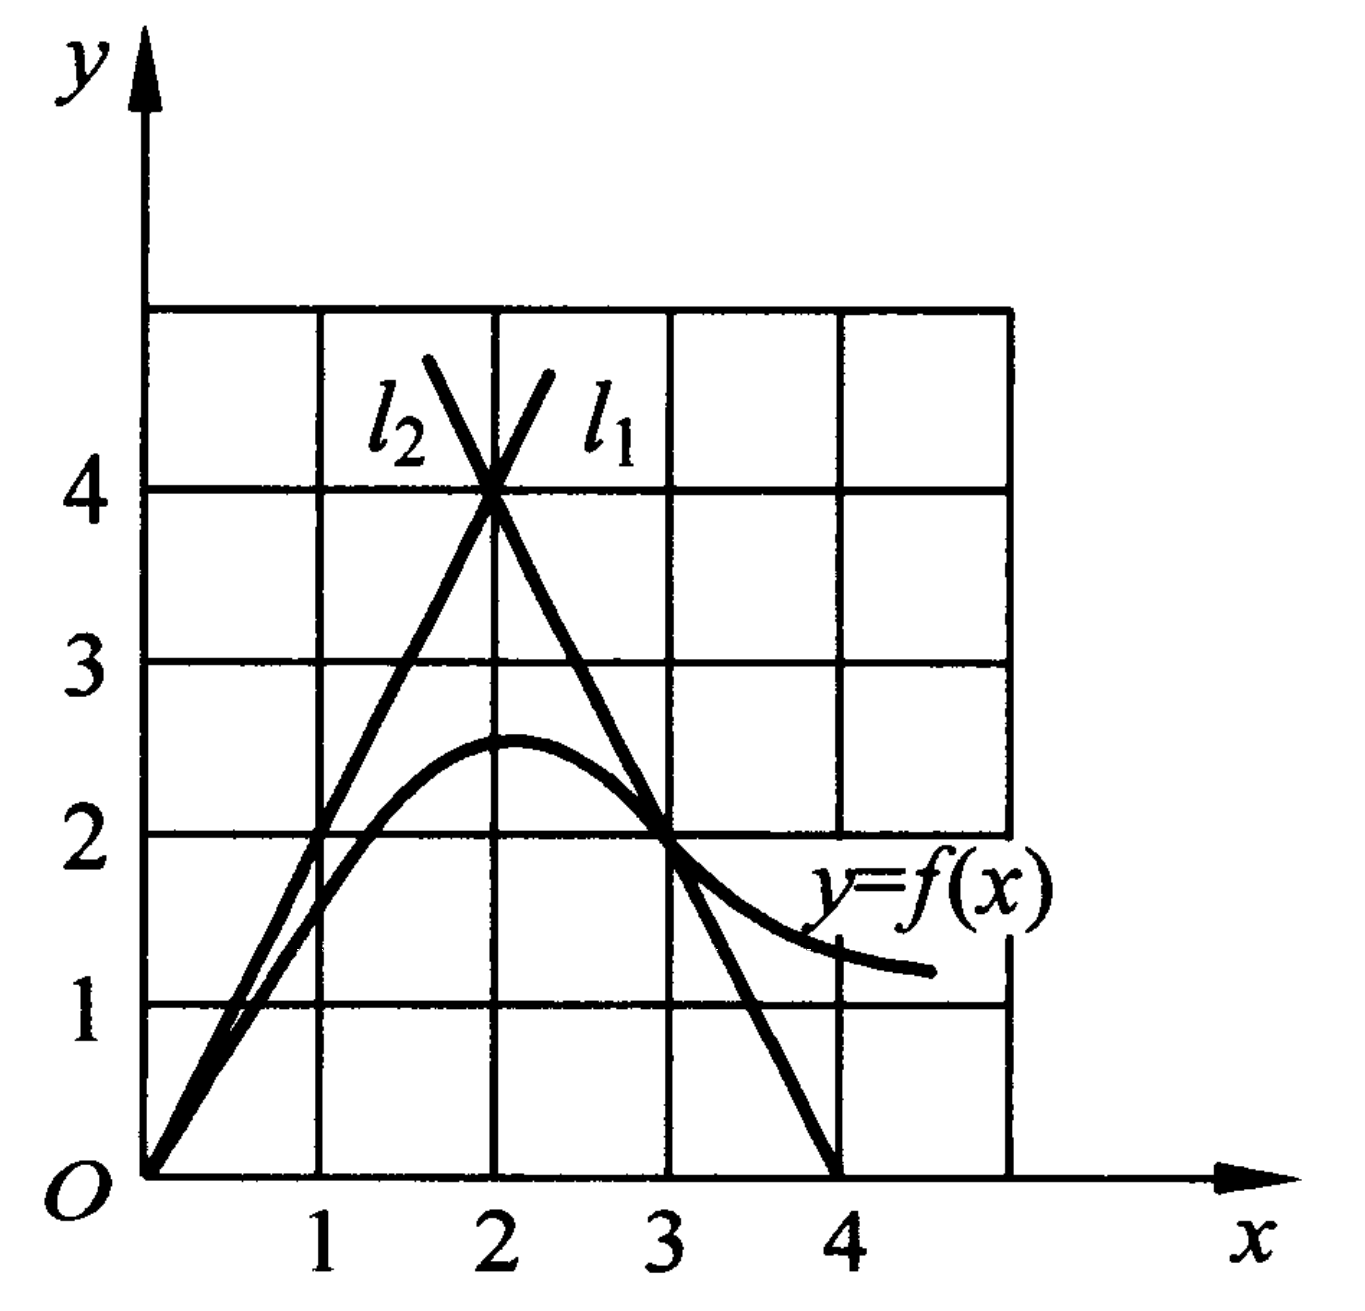
\includegraphics[width=0.5\linewidth]{image/P41-变式3.2-05_1,2.png}
\end{minipage}}
\ansat{263；【方法探究】 - 考点一 - 3.分部积分法 - 变式3.2}

\vspace{6em}
% --- 题目 ---
\problem[P110-变式 (10-2)]{计算二重积分
\[ I = \iint_D r^2 \sin\theta \sqrt{1 - r^2 \cos 2\theta} \, \mathrm{d}r \, \mathrm{d}\theta, \]
其中
\[ D = \left\{(r,\theta) \left| 0 \le r \le \sec \theta, 0 \le \theta \le \frac{\pi}{4} \right.\right\}. \]}
\ansat{306；【方法探究】 - 考点三：二次积分的积分次序与坐标系的转换 - 变式}

% --- 题目 ---
\problem[P4-2 (25-2)]{$\displaystyle \lim_{n \to \infty} \frac{1}{n^2} \left[ \ln \frac{1}{n} + 2\ln \frac{2}{n} + \dots + (n-1)\ln \frac{n-1}{n} \right] = \underline{\hspace{3em}}.$}
\ansat{239；【十年真题】 - 考点二：数列极限的计算 - 2}

% --- 题目 ---
\problem[P222-1 (22-1)]{设随机变量 $\displaystyle X_1, X_2, \dots, X_n$ 独立同分布. 且 $\displaystyle X_1$ 的 $\displaystyle 4$ 阶矩存在. 记 $\displaystyle \mu_k = E(X_1^k) \ (k=1,2,3,4)$, 则根据切比雪夫不等式, 对任意 $\displaystyle \varepsilon > 0$, 有
\[ P\left\{\left|\frac{1}{n}\sum_{i=1}^n X_i^2 - \mu_2\right| \ge \varepsilon\right\} \le (\quad) \]
}
\begin{tasks}(4)
  \task $\displaystyle \frac{\mu_4 - \mu_2^2}{n\varepsilon^2}$.
  \task $\displaystyle \frac{\mu_4 - \mu_2^2}{\sqrt{n}\varepsilon^2}$.
  \task $\displaystyle \frac{\mu_2 - \mu_1^2}{n\varepsilon^2}$.
  \task $\displaystyle \frac{\mu_2 - \mu_1^2}{\sqrt{n}\varepsilon^2}$.
\end{tasks}
\ansat{368；【十年真题】 - 考点：大数定律、中心极限定理与切比雪夫不等式 - 1}

% --- 题目 ---
\problem[P44-5 (20-2)]{设函数 $\displaystyle f(x)$ 的定义域为 $\displaystyle (0, +\infty)$ 且满足
$\displaystyle 2f(x) + x^2 f\left(\frac{1}{x}\right) = \frac{x^2+2x}{\sqrt{1+x^2}}. $
求 $\displaystyle f(x)$, 并求曲线 $\displaystyle y=f(x)$, $\displaystyle y=\frac{1}{2}$, $\displaystyle y=\frac{\sqrt{3}}{2}$ 及 $\displaystyle y$ 轴所围图形绕 $\displaystyle x$ 轴旋转所成旋转体的体积.}
\ansat{267；【十年真题】 - 考点二：平面图形的面积与旋转体的体积 - 5}

\vspace{10em}
% --- 题目 ---
\problem[P52-1 (25-1)]{设函数 $\displaystyle f(x)$ 在区间 $\displaystyle [0, +\infty)$ 上可导, 则 ( \quad )
\begin{tasks}(1)
  \task 当 $\displaystyle \lim_{x \to +\infty} f(x)$ 存在时, $\displaystyle \lim_{x \to +\infty} f'(x)$ 存在.
  \task 当 $\displaystyle \lim_{x \to +\infty} f'(x)$ 存在时, $\displaystyle \lim_{x \to +\infty} f(x)$ 存在.
  \task 当 $\displaystyle \lim_{x \to +\infty} \frac{\int_0^x f(t)\mathrm{d}t}{x}$ 存在时, $\displaystyle \lim_{x \to +\infty} f(x)$ 存在.
  \task 当 $\displaystyle \lim_{x \to +\infty} f(x)$ 存在时, $\displaystyle \lim_{x \to +\infty} \frac{\int_0^x f(t)\mathrm{d}t}{x}$ 存在.
\end{tasks}}
\ansat{270；【十年真题】 - 考点二：含变限积分的函数的极限问题 - 1}

% --- 题目 ---
\problem[P14-3 (07-1,3)]{曲线 $\displaystyle y = \frac{1}{x} + \ln(1 + \mathrm{e}^x)$ 渐近线的条数为~(~\quad~)}
\begin{tasks}(4)
\task 0.
\task 1.
\task 2.
\task 3.
\end{tasks}
\ansat{245；【真题精选】 - 考点二：平面曲线的渐近线 - 3}

% --- 题目 ---
\problem[P69-5 (17-1)]{微分方程 $\displaystyle y'' + 2y' + 3y = 0$ 的通解为 $\displaystyle y = \underline{\hspace{4em}}. $}
\ansat{282；【十年真题】 - 考点二：高阶微分方程的求解 - 5}

% --- 题目 ---
\problem[P14-6 (95-2)]{设 $\displaystyle f(x)$ 和 $\displaystyle \varphi(x)$ 在 $\displaystyle (-\infty, +\infty)$ 上有定义, $\displaystyle f(x)$ 为连续函数, 且 $\displaystyle f(x) \neq 0$, $\displaystyle \varphi(x)$ 有间断点, 则~(~\quad~)}
\begin{tasks}(2)
\task $\displaystyle \varphi[f(x)]$ 必有间断点.
\task $\displaystyle [\varphi(x)]^2$ 必有间断点.
\task $\displaystyle f[\varphi(x)]$ 必有间断点.
\task $\displaystyle \frac{\varphi(x)}{f(x)}$ 必有间断点.
\end{tasks}
\ansat{246；【真题精选】 - 考点三：函数的连续性与间断点 - 6}

% --- 题目 ---
\problem[P160-变式 (04-1)]{设有齐次线性方程组
\[ \begin{cases}
(1+a)x_1 + x_2 + \cdots + x_n = 0, \\
2x_1 + (2+a)x_2 + \cdots + 2x_n = 0, \\
\vdots \\
nx_1 + nx_2 + \cdots + (n+a)x_n = 0
\end{cases} (n \ge 2), \]
试问 $\displaystyle a$ 为何值时, 该方程组有非零解, 并求出其通解.}
\ansat{329；【方法探究】 - 考点一：线性方程组的解的情况及求解 - 变式}

% --- 题目 ---
\problem[P87-2 (25-3)]{已知函数 $\displaystyle z = z(x,y)$ 由 $\displaystyle z + \ln z - \int_y^x x \mathrm{e}^{-t^2} \mathrm{d}t = 1$ 确定, 则 $\displaystyle \left. \frac{\partial^2 z}{\partial x^2} \right|_{(1,1)} = \underline{\hspace{4em}}. $}
\ansat{292；【十年真题】 - 考点二：多元隐函数的偏导数与全微分的计算 - 2}

% --- 题目 ---
\problem[P55-例5 (95-2)]{设 $\displaystyle f(x) = \int_0^x \frac{\sin t}{\pi - t} \mathrm{d}t$， 计算 $\displaystyle \int_0^\pi f(x) \mathrm{d}x$.}
\ansat{55；【方法探究】 - 考点三：变限积分与其他问题的综合 - 4. 求二次积分 - 例5}

% --- 题目 ---
\problem[P199-14 (89-1)]{甲、乙两人独立地对同一目标射击一次, 其命中率分别为 $\displaystyle 0.6$ 和 $\displaystyle 0.5$. 现已知目标被命中, 则它是甲射中的概率为 \underline{\hspace{4em}}.}
\ansat{355；【真题精选】 - 考点一：概率的五大公式 - 14}

% --- 题目 ---
\problem[P26-9 (21-2)]{已知函数 $\displaystyle f(x) = \frac{x|x|}{1+x}$, 求曲线 $\displaystyle y=f(x)$ 的凹凸区间及渐近线.}
\ansat{254；【十年真题】 - 考点二：利用导数判断函数的性质 - 9}

\vspace{6em}
% --- 题目 ---
\problem[P14-4 (07-2)]{函数 $\displaystyle f(x) = \frac{(\mathrm{e}^{\frac{1}{x}} + \mathrm{e})\tan x}{x(\mathrm{e}^{\frac{1}{x}} - \mathrm{e})}$ 在区间 $\displaystyle [-\pi, \pi]$ 上的第一类间断点是 $\displaystyle x=~(~\quad~)$
\begin{tasks}(4)
\task $\displaystyle 0$.
\task $\displaystyle 1$.
\task $\displaystyle -\frac{\pi}{2}$.
\task $\displaystyle \frac{\pi}{2}$.
\end{tasks}}
\ansat{246；【真题精选】 - 考点三：函数的连续性与间断点 - 4}

% --- 题目 ---
\problem[P105-8 (22-1,2,3)]{已知平面区域
\[ D = \left\{(x,y) \left| y-2 \le x \le \sqrt{4-y^2}, 0 \le y \le 2 \right.\right\}, \]
计算 $\displaystyle I = \iint_D \frac{(x-y)^2}{x^2+y^2} \, \mathrm{d}x \, \mathrm{d}y.$}
\ansat{302；【十年真题】 - 考点二：二重积分的计算 - 8}

% --- 题目 ---
\problem[P131-3 (23-1,3)]{已知 $\displaystyle a_n < b_n$ \ ($\displaystyle n = 1, 2, \dots$). 若级数 $\displaystyle \sum_{n=1}^{\infty} a_n$ 与 $\displaystyle \sum_{n=1}^{\infty} b_n$ 均收敛, 则 “$\displaystyle \sum_{n=1}^{\infty} a_n$ 绝对收敛” 是 “$\displaystyle \sum_{n=1}^{\infty} b_n$ 绝对收敛” 的 ( \quad )}
\begin{tasks}(2)
  \task 充分必要条件.
  \task 充分不必要条件.
  \task 必要不充分条件.
  \task 既不充分也不必要条件.
\end{tasks}
\ansat{315；【十年真题】 - 考点：常数项级数的收敛性 - 3}

% --- 题目 ---
\problem[P137-2 (18-3)]{已知 $\displaystyle \cos 2x - \frac{1}{(1+x)^2} = \sum_{n=0}^{\infty} a_n x^n \ (-1 < x < 1)$, 求 $\displaystyle a_n$.}
\ansat{320；【十年真题】 - 考点三：把函数展开成幂级数 - 2}

% --- 题目 ---
\problem[P53-10 (20-2)]{已知函数 $\displaystyle f(x)$ 连续且 $\displaystyle \lim_{x \to 0} \frac{f(x)}{x} = 1, g(x) = \int_0^1 f(xt) \mathrm{d}t$, 求 $\displaystyle g'(x)$ 且证明 $\displaystyle g'(x)$ 在 $\displaystyle x=0$ 处连续.}
\ansat{272；【十年真题】 - 考点三：变限积分与其他问题的综合 - 10}

% --- 题目 ---
\problem[P215-13 (23-1)]{设二维随机变量 $\displaystyle (X, Y)$ 的概率密度为
\[ f(x, y) = \begin{cases} \displaystyle \frac{2}{\pi}(x^2 + y^2), & \displaystyle x^2 + y^2 \le 1, \\ 0, & \text{其他}. \end{cases} \]
\begin{enumerate}
\item[(1)] 求 $\displaystyle X$ 与 $\displaystyle Y$ 的协方差;
\item[(2)] $\displaystyle X$ 与 $\displaystyle Y$ 是否相互独立?
\item[(3)] 求 $\displaystyle Z = X^2 + Y^2$ 的概率密度.
\end{enumerate}}
\begin{note}
  主要错的是 (2)
\end{note}
\ansat{365；【十年真题】 - 考点二：随机变量的协方差与相关系数 - 13}

% --- 题目 ---
\problem[P21-1 (21-1)]{设函数 $\displaystyle f(x)=\frac{\sin x}{1+x^2}$ 在 $\displaystyle x=0$ 处的 3 次泰勒多项式为 $\displaystyle ax+bx^2+cx^3$, 则~(~\quad~)}
\begin{tasks}(2)
\task $\displaystyle a=1, b=0, c=-\frac{7}{6}$.
\task $\displaystyle a=1, b=0, c=\frac{7}{6}$.
\task $\displaystyle a=-1, b=-1, c=-\frac{7}{6}$.
\task $\displaystyle a=-1, b=-1, c=\frac{7}{6}$.
\end{tasks}
\ansat{251；【十年真题】 - 考点二：高阶导数的计算 - 1}

% --- 题目 ---
\problem[P106-17 (17-3)]{计算 $\displaystyle \iint_D \frac{y^3}{(1+x^2+y^4)^2} \mathrm{d}x \, \mathrm{d}y$, 其中 $\displaystyle D$ 是第一象限中以曲线 $\displaystyle y=\sqrt{x}$ 与 $\displaystyle x$ 轴为边界的无界区域.}
\ansat{304；【十年真题】 - 考点二：二重积分的计算 - 17}

% --- 题目 ---
\problem[P196-11 (18-3)]{设随机事件 $\displaystyle A, B, C$ 相互独立, 且}
\[ P(A) = P(B) = P(C) = \frac{1}{2}, \]
{则 $\displaystyle P(AC|A \cup B) = \underline{\hspace{4em}}.$}
\ansat{354；【十年真题】 - 考点一：概率的五大公式 - 11}

% --- 题目 ---
\problem[P44-2 (21-3)]{设平面区域 $\displaystyle D$ 由曲线 $\displaystyle y=\sqrt{x} \sin \pi x$ ($\displaystyle 0 \le x \le 1$) 与 $\displaystyle x$ 轴围成, 则 $\displaystyle D$ 绕 $\displaystyle x$ 轴旋转所成旋转体的体积为 \underline{\hspace{4em}}.}
\ansat{263；【十年真题】 - 考点二 - 3.分部积分法 - 变式3.2}

% --- 题目 ---
\problem[P163-2 (23-1)]{已知 $\displaystyle n$ 阶矩阵 $\displaystyle \bm{A}, \bm{B}, \bm{C}$ 满足 $\displaystyle \bm{ABC} = \bm{O}, \bm{E}$ 为 $\displaystyle n$ 阶单位矩阵. 记矩阵
$$ 
\begin{pmatrix} \bm{O} & \bm{A} \\ \bm{BC} & \bm{E} \end{pmatrix}, \; \begin{pmatrix} \bm{AB} & \bm{C} \\ \bm{O} & \bm{E} \end{pmatrix}, \; \begin{pmatrix} \bm{E} & \bm{AB} \\ \bm{AB} & \bm{O} \end{pmatrix}
$$ 
的秩分别为 $\displaystyle r_1, r_2, r_3$, 则~(~\quad~)}
\begin{tasks}(2)
  \task $\displaystyle r_1 \le r_2 \le r_3.$
  \task $\displaystyle r_1 \le r_3 \le r_2.$
  \task $\displaystyle r_3 \le r_1 \le r_2.$
  \task $\displaystyle r_2 \le r_1 \le r_3.$
\end{tasks}
\ansat{333；【十年真题】 - 考点：向量组的线性相关性、线性表示及秩 - 2}

% --- 题目 ---
\problem[P180-2 (24-2)]{设$\displaystyle \bm{A},\bm{B}$为2阶矩阵, 且$\displaystyle \bm{AB}=\bm{BA}$, 则“$\displaystyle \bm{A}$有两个不相等的特征值”是“$\displaystyle \bm{B}$可对角化”的( \quad )
\begin{tasks}(2)
  \task 充分必要条件.
  \task 充分不必要条件.
  \task 必要不充分条件.
  \task 既不充分也不必要条件.
\end{tasks}}
\ansat{341；【十年真题】 - 考点：矩阵的相似和相似对角化 - 2}

% --- 题目 ---
\problem[P6-例1 (2)]{$\displaystyle \lim_{x \to 0} \frac{\sqrt{1+x} - \sqrt{1+\tan x}}{x \tan^2 x} = \underline{\hspace{3em}}.$}
\ansat{6；【方法探究】 - 考点一：函数极限的计算 - 例1 (2)}

% --- 题目 ---
\problem[P10-1 (12-2)]{设 $\displaystyle a_n > 0 \ $ ($\displaystyle n=1,2,\dots$), $\displaystyle S_n = a_1 + a_2 + \dots + a_n$, 则数列 $\displaystyle \{S_n\}$ 有界是数列 $\displaystyle \{a_n\}$ 收敛的( \quad )}
\begin{tasks}(2)
\task 充分必要条件.
\task 充分非必要条件.
\task 必要非充分条件.
\task 既非充分也非必要条件.
\end{tasks}
\ansat{243；【真题精选】 - 考点二：数列极限的计算 - 1}

\vspace{6em}
% --- 题目 ---
\problem[P4-4 (99-2)]{对任意给定的 $\displaystyle \varepsilon \in (0, 1)$，总存在正整数 $\displaystyle N$，当 $\displaystyle n \ge N$ 时，恒有 $\displaystyle |x_n - a| \le 2\varepsilon$" 是数列 $\displaystyle \{x_n\}$ 收敛于 $\displaystyle a$ 的~(~\quad~)}
\begin{tasks}(2)
  \task 充分条件但非必要条件.
  \task 必要条件但非充分条件.
  \task 充分必要条件.
  \task 既非充分条件又非必要条件.
\end{tasks}
\ansat{238；【真题精选】 - 考点：极限的概念与性质 - 4}

% --- 题目 ---
\problem[P39-2 (23-1,2)]{设连续函数 $\displaystyle f(x)$ 满足: $\displaystyle f(x+2) - f(x) = x$, $\displaystyle \int_0^2 f(x) \mathrm{d}x = 0$, 则 $\displaystyle \int_1^3 f(x) \mathrm{d}x = \underline{\hspace{4em}}$.}
\ansat{262；【十年真题】 - 考点二：利用可加性、对称性与几何意义求积分 - 2}

% --- 题目 ---
\problem[P179-6 (96-1)]{设$\displaystyle \bm{A}=\bm{E}-\bm{\xi}\bm{\xi}^{\mathrm{T}}$, 其中$\displaystyle \bm{E}$是$\displaystyle n$阶单位矩阵, $\displaystyle \bm{\xi}$是$n$维非零列向量, $\displaystyle \bm{\xi}^{\mathrm{T}}$是$\displaystyle \bm{\xi}$的转置. 证明:
\begin{enumerate}
\item[(1)] $\displaystyle \bm{A}^2=\bm{A}$的充分条件是$\displaystyle \bm{\xi}^{\mathrm{T}}\bm{\xi}=1$
\item[(2)] 当$\displaystyle \bm{\xi}^{\mathrm{T}}\bm{\xi}=1$时, $\displaystyle \bm{A}$是不可逆矩阵.
\end{enumerate}}
\ansat{341；【真题精选】 - 考点：矩阵的特征值和特征向量 - 6}

% --- 题目 ---
\problem[P93-8 (21-3)]{求函数 $\displaystyle f(x,y) = 2\ln|x| + \frac{(x-1)^2 + y^2}{2x^2}$ 的极值.}
\ansat{296；【十年真题】 - 考点一：多元函数的无条件极值 - 8}

% --- 题目 ---
\problem[P140-例(2) (03-1)]{将函数 $\displaystyle f(x) = \arctan \frac{1-2x}{1+2x}$ 展开成 $x$ 的幂级数, 并求级数 $\displaystyle \sum_{n=0}^{\infty} \frac{(-1)^n}{2n+1}$ 的和.}
\ansat{140；【方法探究】 - 考点一：幂级数的收敛域 - 例(2)}

% --- 题目 ---
\problem[P4-2 (23-3)]{$\displaystyle \lim_{x \to \infty} x^2 \left(2 - x \sin \frac{1}{x} - \cos \frac{1}{x}\right) = \underline{\hspace{3em}}.$}
\ansat{238；【十年真题】 - 考点一：函数极限的计算 - 2}

% --- 题目 ---
\problem[P200-1 (23-3-局部)]{设随机变量 $\displaystyle X$ 的概率密度为 $\displaystyle f(x) = \frac{\mathrm{e}^x}{(1+\mathrm{e}^x)^2}, -\infty < x < +\infty$, 令 $\displaystyle Y = \mathrm{e}^X$.}
\begin{enumerate}
\item[(1)] 求 $\displaystyle X$ 的分布函数;
\item[(2)] 求 $\displaystyle Y$ 的概率密度.
\end{enumerate}
\begin{note}
  主要错的是 (2)
\end{note}
\ansat{355；【十年真题】 - 考点二：随机变量的函数的分布 - 1}

% --- 题目 ---
\problem[P173-10 (05-1,2)]{已知3阶矩阵$\displaystyle \bm{A}$的第一行是$\displaystyle (a,b,c)$, $\displaystyle a,b,c$不全为零,矩阵 $\displaystyle \bm{B}=\begin{pmatrix} 1 & 2 & 3 \\ 2 & 4 & 6 \\ 3 & 6 & k \end{pmatrix}$ ($\displaystyle k$为常数), 且$\displaystyle \bm{AB}=\bm{O}$, 求线性方程组$\displaystyle \bm{A}\bm{x}=\bm{0}$的通解.}
\ansat{338；【真题精选】 - 考点：线性方程组的解的结构 - 10}

% --- 题目 ---
\problem[P93-4 (23-1)]{求函数 $\displaystyle f(x,y) = (y - x^2)(y - x^3)$ 的极值.}
\ansat{295；【十年真题】 - 考点一：多元函数的无条件极值 - 4}

% --- 题目 ---
\problem[P136-2 (20-3)]{设幂级数 $\displaystyle \sum_{n=1}^{\infty} na_n (x-2)^n$ 的收敛区间为 $(-2, 6)$, 则 $\displaystyle \sum_{n=1}^{\infty} a_n (x+1)^{2n}$ 的收敛区间为 ( \quad )
\begin{tasks}(4)
\task $(-2, 6).$
\task $(-3, 1).$
\task $(-5, 3).$
\task $(-17, 15).$
\end{tasks}}
\ansat{317；【十年真题】 - 考点一：幂级数的收敛域 - 2}

% --- 题目 ---
\problem[P105-11 (20-2)]{设平面区域 $\displaystyle D$ 由 $\displaystyle x=1, x=2, y=x$ 与 $\displaystyle x$ 轴围成,
计算
\[ \iint_D \frac{\sqrt{x^2+y^2}}{x} \mathrm{d}x \, \mathrm{d}y. \]}
\ansat{303；【十年真题】 - 考点二：二重积分的计算 - 11}

\vspace{2em}
% --- 题目 ---
\problem[P11-3 (23-2)]{已知数列 $\displaystyle \{x_n\}, \{y_n\}$ 满足 $\displaystyle x_1 = y_1 = \frac{1}{2}, \ x_{n+1} = \sin x_n, \ y_{n+1} = y_n^2 \ (n=1, 2, \dots)$, 则当 $\displaystyle n \to \infty$ 时~(~\quad~)}
\begin{tasks}(2)
\task $\displaystyle x_n$ 是 $\displaystyle y_n$ 的高阶无穷小.
\task $\displaystyle y_n$ 是 $\displaystyle x_n$ 的高阶无穷小.
\task $\displaystyle x_n$ 与 $\displaystyle y_n$ 是等价无穷小.
\task $\displaystyle x_n$ 与 $\displaystyle y_n$ 是同阶但不等价的无穷小.
\end{tasks}
\ansat{244；【十年真题】 - 考点一：无穷小的比较 - 3}

% --- 题目 ---
\problem[P15-1 (20-3)]{设 $\displaystyle \lim_{x \to a} \frac{f(x)-a}{x-a} = b$, 则 $\displaystyle \lim_{x \to a} \frac{\sin f(x) - \sin a}{x-a} =~(~\quad~)$
\begin{tasks}(2)
\task $\displaystyle b \sin a$.
\task $\displaystyle b \cos a$.
\task $\displaystyle b \sin f(a)$.
\task $\displaystyle b \cos f(a)$.
\end{tasks}}
\ansat{247；【十年真题】 - 考点一：已知极限求另一极限 - 1}

% --- 题目 ---
\problem[P9-15 (08-3)]{计算 \[ \displaystyle \lim_{x \to 0} \frac{1}{x^2} \ln \frac{\sin x}{x}. \]}
\ansat{242；【真题精选】 - 考点一：函数极限的计算 - 15}

% --- 题目 ---
\problem[P34-1 (22-1,2,3)]{设 $\displaystyle I_1 = \int_0^1 \frac{x}{2(1+\cos x)} \mathrm{d}x, I_2 = \int_0^1 \frac{\ln(1+x)}{1+\cos x} \mathrm{d}x$, $\displaystyle I_3 = \int_0^1 \frac{2x}{1+\sin x} \mathrm{d}x$, 则 $( \quad )$
\begin{tasks}(2)
  \task $\displaystyle I_1 < I_2 < I_3$.
  \task $\displaystyle I_2 < I_1 < I_3$.
  \task $\displaystyle I_1 < I_3 < I_2$.
  \task $\displaystyle I_3 < I_2 < I_1$.
\end{tasks}}
\ansat{259；【十年真题】 - 考点二：定积分的概念与性质 - 1}

\vspace{8em}
% --- 题目 ---
\problem[P136-1 (20-1)]{设 $\displaystyle R$ 为幂级数 $\displaystyle \sum_{n=1}^{\infty} a_n x^n$ 的收敛半径, $\displaystyle r$ 是实数, 则 ( \quad )}
\begin{tasks}(2)
\task 当 $\displaystyle \sum_{n=1}^{\infty} a_{2n} r^{2n}$ 发散时, $\displaystyle |r| \ge R$.
\task 当 $\displaystyle \sum_{n=1}^{\infty} a_{2n} r^{2n}$ 收敛时, $\displaystyle |r| \le R$.
\task 当 $\displaystyle |r| \ge R$ 时, $\displaystyle \sum_{n=1}^{\infty} a_{2n} r^{2n}$ 发散.
\task 当 $\displaystyle |r| \le R$ 时, $\displaystyle \sum_{n=1}^{\infty} a_{2n} r^{2n}$ 收敛.
\end{tasks}
\ansat{317；【十年真题】 - 考点一：幂级数的收敛域 - 1}

% --- 题目 ---
\problem[P2-2 (22-1,2)]{设数列 $\displaystyle \{x_n\}$ 满足 $\displaystyle -\frac{\pi}{2} \leqslant x_n \leqslant \frac{\pi}{2}$, 则~(~\quad~)}
\begin{tasks}(1)
  \task 当 $\displaystyle \lim_{n \to \infty} \cos(\sin x_n)$ 存在时, $\displaystyle \lim_{n \to \infty} x_n$ 存在.
  \task 当 $\displaystyle \lim_{n \to \infty} \sin(\cos x_n)$ 存在时, $\displaystyle \lim_{n \to \infty} x_n$ 存在.
  \task 当 $\displaystyle \lim_{n \to \infty} \cos(\sin x_n)$ 存在时, $\displaystyle \lim_{n \to \infty} \sin x_n$ 存在, 但 $\displaystyle \lim_{n \to \infty} x_n$ 不一定存在.
  \task 当 $\displaystyle \lim_{n \to \infty} \sin(\cos x_n)$ 存在时, $\displaystyle \lim_{n \to \infty} \cos x_n$ 存在, 但 $\displaystyle \lim_{n \to \infty} x_n$ 不一定存在.
\end{tasks}
\ansat{238；【十年真题】 - 考点：极限的概念与性质 - 2}

% --- 题目 ---
\problem[P52-6 (19-2)]{已知函数 $\displaystyle f(x) = x \int_1^x \frac{\sin t^2}{t} \mathrm{d}t$, 则 $\displaystyle \int_0^1 f(x) \mathrm{d}x = \underline{\hspace{4em}}. $}
\ansat{272；【十年真题】 - 考点三：变限积分与其他问题的综合 - 6}

% --- 题目 ---
\problem[P2-1 (24-2)]{已知数列 $\displaystyle \{a_n\}$ ($\displaystyle a_n \neq 0$). 若 $\displaystyle \{a_n\}$ 发散, 则~(~\quad~)}
\begin{tasks}(2)
  \task $\displaystyle \left\{a_n + \frac{1}{a_n}\right\}$ 发散.
  \task $\displaystyle \left\{a_n - \frac{1}{a_n}\right\}$ 发散.
  \task $\displaystyle \left\{\mathrm{e}^{a_n} + \frac{1}{\mathrm{e}^{a_n}}\right\}$ 发散.
  \task $\displaystyle \left\{\mathrm{e}^{a_n} - \frac{1}{\mathrm{e}^{a_n}}\right\}$ 发散.
\end{tasks}
\ansat{238；【十年真题】 - 考点：极限的概念与性质 - 1}

\vspace{4em}
% --- 题目 ---
\problem[P69-6 (24-2)]{设 $\displaystyle y(x)$ 为微分方程 $\displaystyle x^2 y'' + xy' - 9y = 0$ 满足条件 $\displaystyle \left.y\right|_{x=1}=2, \left.y'\right|_{x=1}=6$ 的解.
\begin{enumerate}
\item[(1)] 利用变换 $\displaystyle x=\mathrm{e}^t$ 将上述方程化为常系数线性方程, 并求 $\displaystyle y(x)$;
\item[(2)] 计算 $\displaystyle \int_1^2 y(x) \sqrt{4-x^2} \, \mathrm{d}x$.
\end{enumerate}}
\ansat{282；【十年真题】 - 考点二：高阶微分方程的求解 - 6}

% --- 题目 ---
\problem[P8-变式 3 (98-1)]{求极限 $$\lim_{n \to \infty} \left( \frac{\sin \frac{\pi}{n}}{n+1} + \frac{\sin \frac{2\pi}{n}}{n + \frac{1}{2}} + \dots + \frac{\sin \pi}{n + \frac{1}{n}} \right).$$}
\ansat{240；【方法探究】 - 考点二：数列极限的计算 - 变式 3}

% --- 题目 ---
\problem[P26-2 (22-2)]{设函数 $\displaystyle f(x)$ 在 $\displaystyle x=x_0$ 处具有 2 阶导数, 则~(~\quad~)}
\begin{tasks}(1)
  \task 当 $\displaystyle f(x)$ 在 $\displaystyle x_0$ 的某邻域内单调增加时, $\displaystyle f'(x_0)>0$.
  \task 当 $\displaystyle f'(x_0)>0$ 时, $\displaystyle f(x)$ 在 $\displaystyle x_0$ 的某邻域内单调增加.
  \task 当 $\displaystyle f(x)$ 在 $\displaystyle x_0$ 的某邻域内是凹函数时, $\displaystyle f''(x_0)>0$.
  \task 当 $\displaystyle f''(x_0)>0$ 时, $\displaystyle f(x)$ 在 $\displaystyle x_0$ 的某邻域内是凹函数.
\end{tasks}
\ansat{254；【十年真题】 - 考点二：利用导数判断函数的性质 - 2}

% --- 题目 ---
\problem[P104-4 (24-1)]{已知平面区域
\[ D = \left\{(x,y) \left| \sqrt{1-y^2} \le x \le 1, -1 \le y \le 1 \right.\right\}, \]
计算 $\displaystyle \iint_D \frac{x}{\sqrt{x^2+y^2}} \mathrm{d}x \, \mathrm{d}y.$}
\ansat{301；【十年真题】 - 考点二：二重积分的计算 - 4}

\vspace{6em}
% --- 题目 ---
\problem[P106-18 (16-1)]{已知平面区域
\[ D = \left\{(r,\theta) \left| 2 \le r \le 2(1 + \cos\theta), -\frac{\pi}{2} \le \theta \le \frac{\pi}{2} \right.\right\}, \]
计算二重积分
\[ \iint_D x \, \mathrm{d}x \, \mathrm{d}y. \]}
\ansat{304；【十年真题】 - 考点二：二重积分的计算 - 15}

% --- 题目 ---
\problem[P134-变式3 (04-1)]{设有方程 $\displaystyle x^n + nx - 1 = 0$, 其中 $\displaystyle n$ 为正整数. 证明此方程存在唯一正实根 $\displaystyle x_n$, 并证明当 $\displaystyle \alpha > 1$ 时, 级数 $\displaystyle \sum_{n=1}^{\infty} x_n^\alpha$ 收敛.}
\ansat{316；【方法探究】 - 考点：常数项级数的收敛性 - 变式3}

% --- 题目 ---
\problem[P34-1 (24-2)]{设非负函数 $\displaystyle f(x)$ 在 $\displaystyle [0, +\infty)$ 上连续, 给出以下三个命题:
\begin{enumerate}
\item[\textcircled{1}] 若 $\displaystyle \int_0^{+\infty} f^2(x) \mathrm{d}x$ 收敛, 则 $\displaystyle \int_0^{+\infty} f(x) \mathrm{d}x$ 收敛.
\item[\textcircled{2}] 若存在 $\displaystyle p > 1$, 使得 $\displaystyle \lim_{x \to +\infty} x^p f(x)$ 存在, 则 $\displaystyle \int_0^{+\infty} f(x) \mathrm{d}x$ 收敛.
\item[\textcircled{3}] 若 $\displaystyle \int_0^{+\infty} f(x) \mathrm{d}x$ 收敛, 则存在 $\displaystyle p > 1$, 使得 $\displaystyle \lim_{x \to +\infty} x^p f(x)$ 存在.
\end{enumerate}
其中真命题的个数为 ( \quad )
\begin{tasks}(4)
  \task 0.
  \task 1.
  \task 2.
  \task 3.
\end{tasks}}
\ansat{259；【十年真题】 - 考点三：反常积分的收敛性 - 1}

% --- 题目 ---
\problem[P41-变式 3.1 (03-2)]{计算不定积分$\displaystyle \int \frac{x \mathrm{e}^{\arctan x}}{(1+x^2)^{\frac{3}{2}}} \mathrm{d}x$.}
\ansat{263；【方法探究】 - 考点一 - 3.分部积分法 - 变式3.1}

\vspace{8em}
% --- 题目 ---
\problem[P219-12 (15-1,3)]{设随机变量 $\displaystyle X$ 的概率密度为
\[ f(x) = \begin{cases} 2^{-x} \ln 2, & x > 0, \\ 0, & x \le 0. \end{cases} \]
对 $\displaystyle X$ 进行独立重复的观测, 直到第 2 个大于 3 的观测值出现时停止, 记 $\displaystyle Y$ 为观测次数.
\begin{enumerate}
\item[(1)] 求 $\displaystyle Y$ 的概率分布;
\item[(2)] 求 $\displaystyle EY$.
\end{enumerate}}
\begin{note}
  主要错的是 (2)
\end{note}
\ansat{366；【真题精选】 - 考点一：随机变量的数学期望与方差 - 12}

% --- 题目 ---
\problem[P93-6 (22-2)]{已知可微函数 $\displaystyle f(u,v)$ 满足
\[ \frac{\partial f(u,v)}{\partial u} - \frac{\partial f(u,v)}{\partial v} = 2(u-v)\mathrm{e}^{-(u+v)}, \]
且 $\displaystyle f(u,0) = u^2 \mathrm{e}^{-u}$.
\begin{enumerate}
\item[(1)] 记 $\displaystyle g(x,y) = f(x, y-x)$, 求 $\displaystyle \frac{\partial g(x,y)}{\partial x}$;
\item[(2)] 求 $\displaystyle f(u,v)$ 的表达式和极值.
\end{enumerate}}
\ansat{296；【十年真题】 - 考点一：多元函数的无条件极值 - 6}

% --- 题目 ---
\problem[P77-16 (18-1)]{已知微分方程 $\displaystyle y'+y=f(x)$, 其中 $\displaystyle f(x)$ 是 $\displaystyle \mathbb{R}$ 上的连续函数.
\begin{enumerate}
\item[(1)] 若 $\displaystyle f(x)=x$, 求方程的通解;
\item[(2)] 若 $\displaystyle f(x)$ 是周期为 $\displaystyle T$ 的函数, 证明: 方程存在唯一的以 $\displaystyle T$ 为周期的解.
\end{enumerate}}
\begin{note}
    主要错的是 (2)
\end{note}
\ansat{286；【十年真题】 - 考点：微分方程的应用 - 16}

% --- 题目 ---
\problem[P24-例(2)]{设函数 $\displaystyle y=x^2 \sin 2x$, 则 $\displaystyle y^{(5)}(0) = \underline{\hspace{4em}}. $}
\ansat{24；【方法探究】 - 考点二：高阶导数的计算 - 例(2)}

\vspace{5em}
% --- 题目 ---
\problem[P108-例 (09-1)]{如下图所示, 正方形 $\displaystyle \{(x,y) \mid |x| \le 1, |y| \le 1\}$ 被其对角线划分为四个区域 $\displaystyle D_k \ (k = 1,2,3,4)$, $\displaystyle I_k = \iint_{D_k} y \cos x \, \mathrm{d}x \, \mathrm{d}y$, 则 $\displaystyle \max_{1 \le k \le 4} \{I_k\} = (\quad)$. \\
\begin{minipage}[c]{0.7\textwidth} % 左侧文字和公式区域，宽度占 60%
\begin{tasks}(4)
  \task $\displaystyle I_1$.
  \task $\displaystyle I_2$.
  \task $\displaystyle I_3$.
  \task $\displaystyle I_4$.
\end{tasks}
\end{minipage}
\hfill % 弹性间隔，将左右两个 minipage 推开
\begin{minipage}[c]{0.3\textwidth} % 右侧图片区域，宽度占 35%
\centering % 图片居中
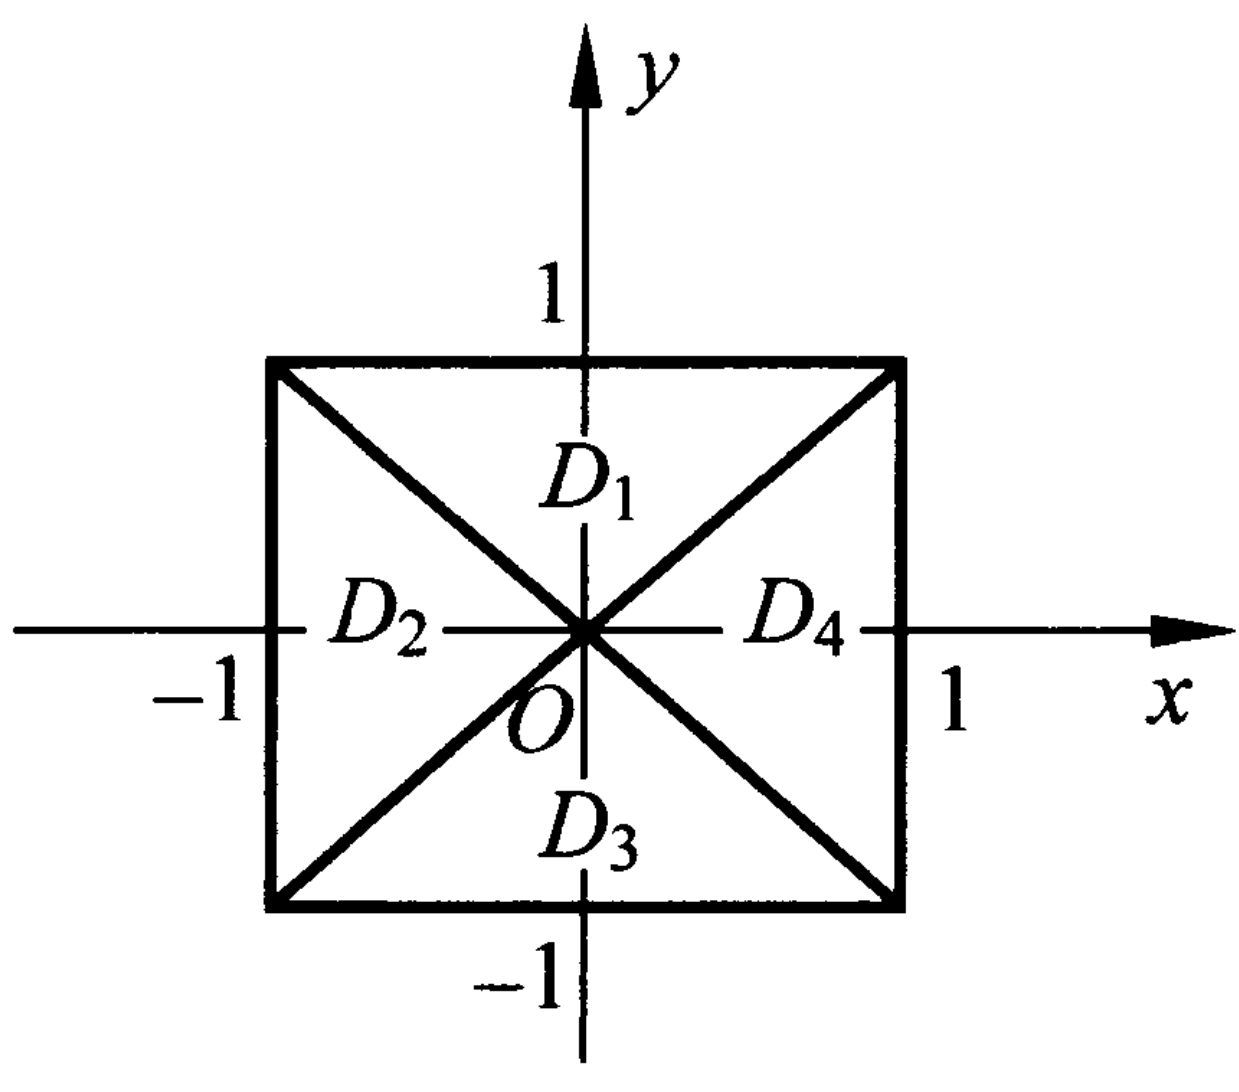
\includegraphics[width=0.5\linewidth]{image/P108-09_1.png}
\end{minipage}}
\ansat{109；【方法探究】 - 考点一：二重积分的概念与性质 - 例}

% --- 题目 ---
\problem[P7-变式 1.1 (97-2)]{求极限 $\displaystyle \lim_{x \to -\infty} \frac{\sqrt{4x^2+x-1}+x+1}{\sqrt{x^2+\sin x}}$.}
\ansat{240；【方法探究】 - 考点一：函数极限的计算 - 变式 1.1}

% --- 题目 ---
\problem[P9-8 (97-1)]{$\displaystyle \lim_{x \to 0} \frac{3\sin x + x^2 \cos \frac{1}{x}}{(1 + \cos x)\ln(1 + x)} = \underline{\hspace{4em}}. $}
\ansat{241；【真题精选】 - 考点一：函数极限的计算 - 8}

% --- 题目 ---
\problem[P71-例(3) (90-2)]{微分方程 $\displaystyle x \ln x \, \mathrm{d}y + (y - \ln x) \, \mathrm{d}x = 0$ 满足条件 $\displaystyle \left.y\right|_{x=\mathrm{e}} = 1$ 的特解是 $\displaystyle y = \underline{\hspace{4em}}. $}
\ansat{71；【方法探究】 - 考点一：一阶微分方程的求解 - 例(3)}

% --- 题目 ---
\problem[P227-5 (08-1,3)]{设 $\displaystyle X_1, X_2, \dots, X_n$ 是总体 $\displaystyle N(\mu, \sigma^2)$ 的简单随机样本. 记 $\displaystyle \bar{X} = \frac{1}{n} \sum_{i=1}^n X_i, S^2 = \frac{1}{n-1} \sum_{i=1}^n (X_i - \bar{X})^2, \ T = \bar{X}^2 - \frac{1}{n} S^2$.
\begin{enumerate}
\item[(1)] 证明 $\displaystyle ET = \mu^2$;
\item[(2)] 当 $\displaystyle \mu=0, \sigma=1$ 时, 求 $\displaystyle DT$.
\end{enumerate}}
\begin{note}
  主要错的是 (2)
\end{note}
\ansat{371；【真题精选】 - 考点二：统计量的数字特征 - 5}

% --- 题目 ---
\problem[P146-4 (20-1,2,3)]{行列式 $\displaystyle \begin{vmatrix} a & 0 & -1 & 1 \\ 0 & a & 1 & -1 \\ -1 & 1 & a & 0 \\ 1 & -1 & 0 & a \end{vmatrix} = \underline{\hspace{4em}}.$}
\ansat{323；【十年真题】 - 考点：具体行列式的计算 - 4}

% --- 题目 ---
\problem[P215-12 (20-1)]{设 $\displaystyle X$ 服从区间 $\displaystyle \left(-\frac{\pi}{2}, \frac{\pi}{2}\right)$ 上的均匀分布, $\displaystyle Y = \sin X$, 则 $\displaystyle \mathrm{Cov}(X, Y) = \underline{\hspace{4em}}. $}
\ansat{365；【十年真题】 - 考点二：随机变量的协方差与相关系数 - 12}

% --- 题目 ---
\problem[P134-例3 (97-1)]{设 $\displaystyle a_1 = 2, a_{n+1} = \frac{1}{2} \left(a_n + \frac{1}{a_n}\right)$ \ ($\displaystyle n = 1, 2, \dots$), 证明:
\begin{enumerate}
\item[(1)] $\displaystyle \lim_{n \to \infty} a_n$ 存在;
\item[(2)] 级数 $\displaystyle \sum_{n=1}^{\infty} \left(\frac{a_n}{a_{n+1}} - 1\right)$ 收敛.
\end{enumerate}}
\ansat{134；【方法探究】 - 考点：常数项级数的收敛性 - 例3}

% --- 题目 ---
\problem[P136-6 (21-1)]{设 $\displaystyle u_n(x) = \mathrm{e}^{-nx} + \frac{x^{n+1}}{n(n+1)} \ (n = 1, 2, \cdots)$, 求级数 $\displaystyle \sum_{n=1}^{\infty} u_n(x)$ 的收敛域及和函数.}
\ansat{318；【十年真题】 - 考点二：幂级数的和函数 - 6}

% --- 题目 ---
\problem[P131-1 (25-1)]{已知级数：\textcircled{1} $\displaystyle \sum_{n=1}^{\infty} \sin \frac{n^3 \pi}{n^2+1}$； \textcircled{2} $\displaystyle \sum_{n=1}^{\infty} (-1)^n \left(\frac{1}{\sqrt[3]{n^2}} - \tan \frac{1}{\sqrt[3]{n^2}}\right)$, 则 ( \quad )
\begin{tasks}(2)
  \task \textcircled{1}与\textcircled{2}均条件收敛.
  \task \textcircled{1}条件收敛, \textcircled{2}绝对收敛.
  \task \textcircled{1}绝对收敛, \textcircled{2}条件收敛.
  \task \textcircled{1}与\textcircled{2}均绝对收敛.
\end{tasks}}
\ansat{315；【十年真题】 - 考点：常数项级数的收敛性 - 1}

\vspace{4em}
% --- 题目 ---
\problem[P59-2 (18-2,3)]{设函数 $\displaystyle f(x)$ 在 $\displaystyle [0,1]$ 上二阶可导, 且 $\displaystyle \int_0^1 f(x) \mathrm{d}x = 0$, 则 ( \quad )
\begin{tasks}(2)
  \task 当 $\displaystyle f'(x) < 0$ 时, $\displaystyle f\left(\frac{1}{2}\right) < 0$.
  \task 当 $\displaystyle f''(x) < 0$ 时, $\displaystyle f\left(\frac{1}{2}\right) < 0$.
  \task 当 $\displaystyle f'(x) > 0$ 时, $\displaystyle f\left(\frac{1}{2}\right) < 0$.
  \task 当 $\displaystyle f''(x) > 0$ 时, $\displaystyle f\left(\frac{1}{2}\right) < 0$.
\end{tasks}}
\ansat{276；【十年真题】 - 考点三：不等式问题 - 2}

% --- 题目 ---
\problem[P106-14 (18-2)]{设平面区域 $\displaystyle D$ 由曲线
\[ \begin{cases} x = t - \sin t, \\ y = 1 - \cos t \end{cases} (0 \le t \le 2\pi) \]
与 $\displaystyle x$ 轴围成, 计算二重积分
\[ \iint_D (x + 2y) \mathrm{d}x \, \mathrm{d}y. \]}
\ansat{303；【十年真题】 - 考点二：二重积分的计算 - 14}

% --- 题目 ---
\problem[P4-7 (16-2,3)]{求极限 $\displaystyle \lim_{x \to 0} (\cos 2x + 2x \sin x)^{\frac{1}{x^4}}$.}
\ansat{239；【十年真题】 - 考点一：函数极限的计算 - 7}

% --- 题目 ---
\problem[P149-4 (96-5)]{5 阶行列式 $\displaystyle \begin{vmatrix} 1-a & a & 0 & 0 & 0 \\ -1 & 1-a & a & 0 & 0 \\ 0 & -1 & 1-a & a & 0 \\ 0 & 0 & -1 & 1-a & a \\ 0 & 0 & 0 & -1 & 1-a \end{vmatrix} = \underline{\hspace{4em}}.$}
\ansat{324；【真题精选】 - 考点：具体行列式的计算 - 4}

% --- 题目 ---
\problem[P41-变式2 (91-2)]{$\displaystyle \int_3^{+\infty} \frac{\mathrm{d}x}{(x-1)^4 \sqrt{x^2 - 2x}} = \underline{\hspace{4em}}$.}
\ansat{263；【方法探究】 - 考点一 - 2.换元积分法 - 变式2}

% --- 题目 ---
\problem[P20-3 (05-1,2)]{设函数 $\displaystyle f(x) = \lim_{n \to \infty} \sqrt[n]{1+|x|^{3n}}$, 则 $\displaystyle f(x)$ 在 $\displaystyle (-\infty, +\infty)$ 内~(~\quad~)}
\begin{tasks}(2)
\task 处处可导.
\task 恰有一个不可导点.
\task 恰有两个不可导点.
\task 至少有三个不可导点.
\end{tasks}
\ansat{251；【真题精选】 - 考点：导数与微分的概念 - 3}

% --- 题目 ---
\problem[P137-9 (17-3)]{设 $\displaystyle a_0 = 1, \ a_1 = 0, \ a_{n+1} = \frac{1}{n+1}(na_n + a_{n-1}) \ (n = 1, 2, 3, \ldots), \ S(x)$ 为幂级数 $\displaystyle \sum_{n=0}^{\infty} a_n x^n$ 的和函数.
\begin{enumerate}
\item[(1)] 证明幂级数 $\displaystyle \sum_{n=0}^{\infty} a_n x^n$ 的收敛半径不小于 $1$;
\item[(2)] 证明 $\displaystyle (1-x)S'(x) - xS(x) = 0 \ (x \in (-1, 1))$, 并求 $\displaystyle S(x)$ 的表达式.
\end{enumerate}}
\ansat{319；【十年真题】 - 考点二：幂级数的和函数 - 9}

% --- 题目 ---
\problem[P21-7 (16-1)]{设函数 $\displaystyle f(x) = \arctan x - \frac{x}{1+ax^2}$, 且 $\displaystyle f'''(0) = 1$, 则 $\displaystyle a = \underline{\hspace{4em}}. $}
\ansat{251；【十年真题】 - 考点二：高阶导数的计算 - 7}

% --- 题目 ---
\problem[P53-11 (16-2,3)]{设函数 $\displaystyle f(x) = \int_0^1 |t^2 - x^2| \mathrm{d}t$ ($\displaystyle x > 0$), 求 $\displaystyle f'(x)$, 并求 $\displaystyle f(x)$ 的最小值.}
\ansat{272；【十年真题】 - 考点三：变限积分与其他问题的综合 - 11}

% --- 题目 ---
\problem[P11-6 (20-2)]{求曲线 $\displaystyle y = \frac{x^{1+x}}{(1+x)^x} \ (x > 0)$ 的斜渐近线方程.}
\ansat{244；【十年真题】 - 考点二：平面曲线的渐近线 - 6}

% --- 题目 ---
\problem[P14-8 (00-3)]{求函数 $\displaystyle f(x)=(x-1)\mathrm{e}^{\frac{\pi}{2} + \arctan x}$ 图形的渐近线.}
\ansat{246；【真题精选】 - 考点二：平面曲线的渐近线 - 8}

% --- 题目 ---
\problem[P224-3 (24-3-仅数学三)]{设总体 $\displaystyle X$ 服从 $\displaystyle [0, \theta]$ 上的均匀分布, 其中 $\displaystyle \theta \in (0, +\infty)$ 为未知参数. $\displaystyle X_1, X_2, \dots, X_n$ 是来自总体 $\displaystyle X$ 的简单随机样本, 记 $\displaystyle X_{(n)} = \max\{X_1, X_2, \dots, X_n\}, T_c = cX_{(n)}$.
\begin{enumerate}
\item[(1)] 求 $\displaystyle c$, 使得 $\displaystyle E(T_c) = \theta$;
\item[(2)] 记 $\displaystyle h(c) = E[(T_c - \theta)^2]$, 求 $\displaystyle c$ 使得 $\displaystyle h(c)$ 最小.
\end{enumerate}}
\ansat{370；【十年真题】 - 考点二：统计量的数字特征 - 3}

% --- 题目 ---
\problem[P25-7 (97-3)]{设 $\displaystyle y = f(\ln x) \mathrm{e}^{f(x)}$, 其中 $\displaystyle f$ 可微, 则 $\displaystyle \mathrm{d}y = \underline{\hspace{4em}}. $}
\ansat{252；【真题精选】 - 考点一：函数的求导与微分法则 - 7}

% --- 题目 ---
\problem[P14-2 (12-1,2,3)]{曲线 $\displaystyle y = \frac{x^2+x}{x^2-1}$ 渐近线的条数为~(~\quad~)}
\begin{tasks}(4)
\task 0.
\task 1.
\task 2.
\task 3.
\end{tasks}
\ansat{245；【真题精选】 - 考点二：平面曲线的渐近线 - 2}

% --- 题目 ---
\problem[P131-8 (16-1)]{已知函数 $\displaystyle f(x)$ 可导, 且 $\displaystyle f(0)=1, 0 < f'(x) < \frac{1}{2}$.
设数列 $\displaystyle \{x_n\}$ 满足 $\displaystyle x_{n+1} = f(x_n) \ (n=1, 2, \dots)$. 证明:
\begin{enumerate}
\item[(1)] 级数 $\displaystyle \sum_{n=1}^{\infty} (x_{n+1} - x_n)$ 绝对收敛;
\item[(2)] $\displaystyle \lim_{n \to \infty} x_n$ 存在, 且 $\displaystyle 0 < \lim_{n \to \infty} x_n < 2$.
\end{enumerate}}
\ansat{316；【十年真题】 - 考点：常数项级数的收敛性 - 8}

% --- 题目 ---
\problem[P107-6 (20-2)]{$\displaystyle \int_0^1 \mathrm{d}y \int_{\sqrt{y}}^1 \sqrt{x^3 + 1} \, \mathrm{d}x = \underline{\hspace{4em}}. $}
\ansat{305；【十年真题】 - 考点三：二次积分的积分次序与坐标系的转换 - 6}

% --- 题目 ---
\problem[P69-2 (25-3)]{微分方程 $\displaystyle xy' - y + x^2 \mathrm{e}^x = 0$ 满足 $\displaystyle y(1) = -\mathrm{e}$ 的解为 $\displaystyle y = \underline{\hspace{4em}}. $}
\ansat{281；【十年真题】 - 考点一：一阶微分方程的求解 - 2}

% --- 题目 ---
\problem[P136-2 (23-3)]{$\displaystyle \sum_{n=0}^{\infty} \frac{x^{2n}}{(2n)!} = \underline{\hspace{4em}}.$}
\ansat{318；【十年真题】 - 考点二：幂级数的和函数 - 2}

% --- 题目 ---
\problem[P104-6 (23-2)]{设平面有界区域 $\displaystyle D$ 位于第一象限, 由曲线 $\displaystyle x^2 + y^2 - xy = 1, x^2 + y^2 - xy = 2$ 与直线 $\displaystyle y = \sqrt{3}x, y = 0$ 围成,
计算 $\displaystyle \iint_D \frac{1}{3x^2 + y^2} \mathrm{d}x \, \mathrm{d}y.$}
\ansat{302；【十年真题】 - 考点二：二重积分的计算 - 6}

% --- 题目 ---
\problem[P104-5 (24-2.3)]{设平面有界区域 $\displaystyle D$ 位于第一象限, 由曲线 $\displaystyle xy = \frac{1}{3}$, $\displaystyle xy = 3$ 与直线 $\displaystyle y = \frac{x}{3}, y = 3x$ 围成, 计算 $\displaystyle \iint_D (1+x-y) \mathrm{d}x \, \mathrm{d}y$.}
\ansat{302；【十年真题】 - 考点二：二重积分的计算 - 5}

% --- 题目 ---
\problem[P53-8 (24-2)]{设 $\displaystyle t > 0$, 平面有界区域 $\displaystyle D$ 由曲线 $\displaystyle y=\sqrt{x} \, \mathrm{e}^{-x}$ 与直线 $\displaystyle x=t, x=2t$ 及 $\displaystyle x$ 轴围成, $\displaystyle D$ 绕 $\displaystyle x$ 轴旋转一周所得旋转体的体积为 $\displaystyle V(t)$, 求 $\displaystyle V(t)$ 的最大值.}
\ansat{272；【十年真题】 - 考点三：变限积分与其他问题的综合 - 8}

% --- 题目 ---
\problem[P87-3 (23-2)]{设函数 $\displaystyle z=z(x, y)$ 由方程 $\displaystyle \mathrm{e}^z + xz = 2x - y$ 确定, 则 $\displaystyle \left. \frac{\partial^2 z}{\partial x^2} \right|_{(1,1)} = \underline{\hspace{4em}}. $}
\ansat{292；【十年真题】 - 考点一：多元复合函数的偏导数与全微分的计算 - 3}

\vspace{10em}
% --- 题目 ---
\problem[P180-5 (22-2,3)]{设$\displaystyle \bm{A}$为3阶矩阵, $\displaystyle \bm{\Lambda}=\begin{pmatrix} 1 & 0 & 0 \\ 0 & -1 & 0 \\ 0 & 0 & 0 \end{pmatrix}$, 则$\displaystyle \bm{A}$的特征值为 $\displaystyle 1,-1,0$ 的充分必要条件是( \quad )
\begin{tasks}(2)
  \task 存在可逆矩阵$\displaystyle \bm{P},\bm{Q}$, 使得$\displaystyle \bm{A}=\bm{P}\bm{\Lambda}\bm{Q}$.
  \task 存在可逆矩阵$\displaystyle \bm{P}$, 使得$\displaystyle  \bm{A}=\bm{P}\bm{\Lambda}\bm{P}^{-1}$.
  \task 存在正交矩阵$\displaystyle \bm{Q}$, 使得$\displaystyle \bm{A}=\bm{Q}\bm{\Lambda}\bm{Q}^{-1}$.
  \task 存在可逆矩阵$\displaystyle \bm{P}$, 使得$\displaystyle \bm{A}=\bm{P}\bm{\Lambda}\bm{P}^{\mathrm{T}}$.
\end{tasks}}
\ansat{341；【十年真题】 - 考点：矩阵的相似和相似对角化 - 5}

% --- 题目 ---
\problem[P139-例2 (08-1)]{已知幂级数 $\displaystyle \sum_{n=0}^{\infty} a_n (x+2)^n$ 在 $\displaystyle x = 0$ 处收敛, 在 $\displaystyle x = -4$ 处发散, 则幂级数 $\displaystyle \sum_{n=0}^{\infty} a_n (x-3)^n$ 的收敛域为 \underline{\hspace{4em}}.}
\ansat{139；【方法探究】 - 考点一：幂级数的收敛域 - 例2}

% --- 题目 ---
\problem[P84-4 (20-2)]{关于函数
\[ f(x,y) = \begin{cases} \displaystyle xy, & xy \neq 0, \\ \displaystyle x, & y = 0, \\ \displaystyle y, & x = 0, \end{cases} \]
给出以下结论:
\begin{multicols}{2}
\begin{itemize}
    \setstretch{3}
    \item[\textcircled{1}] $\displaystyle \left. \frac{\partial f}{\partial x} \right|_{(0,0)} = 1$;
    \item[\textcircled{2}] $\displaystyle \left. \frac{\partial^2 f}{\partial x \partial y} \right|_{(0,0)} = 1$;
    \item[\textcircled{3}] $\displaystyle \lim_{(x,y) \to (0,0)} f(x,y) = 0$;
    \item[\textcircled{4}] $\displaystyle \lim_{y \to 0} \lim_{x \to 0} f(x,y) = 0$.
\end{itemize}
\end{multicols}
其中正确的个数为 ( \quad )
\begin{tasks}(4)
\task 4.
\task 3.
\task 2.
\task 1.
\end{tasks}}
\ansat{291；【十年真题】 - 考点：多元函数微分学的基本概念 - 4}

% --- 题目 ---
\problem[P136-4 (17-1)]{幂级数 $\displaystyle \sum_{n=1}^{\infty} (-1)^{n-1} n x^{n-1}$ 在区间 $(-1, 1)$ 内的和函数 $\displaystyle S(x) = \underline{\hspace{4em}}.$}
\ansat{318；【十年真题】 - 考点二：幂级数的和函数 - 4}

% --- 题目 ---
\problem[P93 (22-1)]{若当 $\displaystyle x \ge 0, y \ge 0$ 时, $\displaystyle x^2+y^2 \le k\mathrm{e}^{x+y}$ 恒成立, 则 $\displaystyle k$ 的取值范围是 \underline{\hspace{4em}}.}
\ansat{296；【十年真题】 - 考点三：多元函数在闭区域上的最值}

% --- 题目 ---
\problem[P109-变式2 (08-2,3)]{计算 $\displaystyle \iint_D \max\{xy, 1\} \mathrm{d}x \, \mathrm{d}y$, 其中 $\displaystyle D = \{(x,y) \mid 0 \le x \le 2, 0 \le y \le 2\}$.}
\ansat{305；【方法探究】 - 考点二：二重积分的计算 - 变式2}

% --- 题目 ---
\problem[P215-8 (20-3)]{设随机变量 $\displaystyle (X, Y)$ 服从二维正态分布 $\displaystyle N\left(0, 0; 1, 4; -\frac{1}{2}\right)$, 则下列随机变量中服从标准正态分布且与 $\displaystyle X$ 独立的是~(~\quad~)}
\begin{tasks}(4)
  \task $\displaystyle \frac{\sqrt{5}}{5}(X+Y).$
  \task $\displaystyle \frac{\sqrt{5}}{5}(X-Y).$
  \task $\displaystyle \frac{\sqrt{3}}{3}(X+Y).$
  \task $\displaystyle \frac{\sqrt{3}}{3}(X-Y).$
\end{tasks}
\ansat{364；【十年真题】 - 考点二：随机变量的协方差与相关系数 - 8}

% --- 题目 ---
\problem[P75-4 (20-1)]{设函数 $\displaystyle f(x)$ 满足 $\displaystyle f''(x) + af'(x) + f(x) = 0$ ($\displaystyle a > 0$), 且 $\displaystyle f(0) = m, f'(0) = n$, 则 $\displaystyle \int_0^{+\infty} f(x) \mathrm{d}x = \underline{\hspace{4em}}. $}
\ansat{284；【十年真题】 - 考点：微分方程的应用 - 4}

% --- 题目 ---
\problem[P87-5 (20-1)]{设函数 $\displaystyle f(x,y) = \int_0^{xy} \mathrm{e}^{xt^2} \mathrm{d}t$, 则 $\displaystyle \left. \frac{\partial^2 f}{\partial x \partial y} \right|_{(1,1)} = \underline{\hspace{4em}}. $}
\ansat{291；【十年真题】 - 考点一：多元复合函数的偏导数与全微分的计算 - 5}

% --- 题目 ---
\problem[P10-4 (02-2)]{$\displaystyle \lim_{n \to \infty} \frac{1}{n} \left[ \sqrt{1+\cos \frac{\pi}{n}} + \sqrt{1+\cos \frac{2\pi}{n}} + \ldots + \sqrt{1+\cos \frac{n\pi}{n}} \right] = \underline{\hspace{4em}}. $}
\ansat{243；【真题精选】 - 考点二：数列极限的计算 - 4}

% --- 题目 ---
\problem[P10-2 (04-2)]{$\displaystyle \lim_{n \to \infty} \ln \sqrt[n]{ \left(1+\frac{1}{n}\right)^2 \left(1+\frac{2}{n}\right)^2 \cdots \left(1+\frac{n}{n}\right)^2 }$ 等于~(~\quad~)}
\begin{tasks}(2)
 \task $\displaystyle \int_{1}^{2} \ln^2 x \, \mathrm{d}x.$
 \task $\displaystyle 2 \int_{1}^{2} \ln x \, \mathrm{d}x.$
 \task $\displaystyle 2 \int_{1}^{2} \ln(1+x) \, \mathrm{d}x.$
 \task $\displaystyle \int_{1}^{2} \ln^2(1+x) \, \mathrm{d}x.$
\end{tasks}
\ansat{243；【真题精选】 - 考点二：数列极限的计算 - 2}

% --- 题目 ---
\probtagged[P8-变式 4.1 (96-1)]{设 $\displaystyle x_1 = 10, \ x_{n+1} = \sqrt{6+x_n} \ (n = 1, 2, \dots)$. 试证数列 $\displaystyle \{x_n\}$ 极限存在, 并求此极限.}
\ansat{241；【方法探究】 - 考点二：数列极限的计算 - 变式 4.1}

% --- 题目 ---
\problem[P186-10 (02-1)]{设$\displaystyle \bm{A}, \bm{B}$为同阶方阵.
\begin{enumerate}
\item[(1)] 如果$\displaystyle \bm{A}, \bm{B}$相似, 试证$\displaystyle \bm{A}, \bm{B}$的特征多项式相等;
\end{enumerate}}
\ansat{345；【真题精选】 - 考点：矩阵的相似和相似对角化 - 10}

% --- 题目 ---
\problem[P148-例2 (1)]{$\displaystyle n$ 阶行列式 $\displaystyle \begin{vmatrix} 1 & -1 & & & & \\ 2 & a & -1 & & & \\ 3 & & a & -1 & & \\ \vdots & & \ddots & \ddots & & \\ n-1 & & & & a & -1 \\ n & & & & & a \end{vmatrix} = \underline{\hspace{4em}}.$}
\ansat{148；【方法探究】 - 考点：具体行列式的计算 - 例2 (1)}

\vspace{10em}
% --- 题目 ---
\problem[P133-例1]{下列级数中发散的是 ( \quad )
\begin{tasks}(2)
  \task $\displaystyle \sum_{n=1}^{\infty} \frac{2^n \cdot n!}{n^n}.$
  \task $\displaystyle \sum_{n=1}^{\infty} \left(\frac{1}{\sqrt{n}} - \sin \frac{1}{\sqrt{n}}\right).$
  \task $\displaystyle \sum_{n=1}^{\infty} \left(\frac{n+1}{2n+3}\right)^n \sin(n+1).$
  \task $\displaystyle \sum_{n=2}^{\infty} \left[\frac{1}{n \ln n} - \frac{(-1)^n}{n}\right].$
\end{tasks}}
\ansat{133；【方法探究】 - 考点：常数项级数的收敛性 - 例1}

% --- 题目 ---
\problem[P20-1 (07-1,2,3)]{设函数 $\displaystyle f(x)$ 在 $\displaystyle x=0$ 处连续, 下列命题错误的是~(~\quad~)
\begin{tasks}(2)
\task 若 $\displaystyle \lim_{x \to 0} \frac{f(x)}{x}$ 存在, 则 $\displaystyle f(0)=0$.
\task 若 $\displaystyle \lim_{x \to 0} \frac{f(x)+f(-x)}{x}$ 存在, 则 $\displaystyle f(0)=0$.
\task 若 $\displaystyle \lim_{x \to 0} \frac{f(x)}{x}$ 存在, 则 $\displaystyle f'(0)$ 存在.
\task 若 $\displaystyle \lim_{x \to 0} \frac{f(x)-f(-x)}{x}$ 存在, 则 $\displaystyle f'(0)$ 存在.
\end{tasks}}
\ansat{250；【真题精选】 - 考点：导数与微分的概念 - 1}

% --- 题目 ---
\problem[P139-例2]{设 $\displaystyle a_0 = 1$, $\displaystyle (n+1)a_{n+1} + (n+5)a_n = 0$, \ $\displaystyle S(x)$ 为幂级数 $\displaystyle \sum_{n=0}^{\infty} a_n x^n$ 的和函数.
\begin{enumerate}
\item[(1)] 求 $\displaystyle \sum_{n=0}^{\infty} a_n x^n$ 的收敛区间;
\item[(2)] 求 $\displaystyle S(x)$ 所满足的微分方程, 并求 $\displaystyle S(x)$ 的表达式.
\end{enumerate}}
\ansat{139；【方法探究】 - 考点二：幂级数的和函数 - 例2}

% --- 题目 ---
\problem[P105-7 (23-3)]{已知平面区域 $$\displaystyle D = \left\{(x,y) \left| (x-1)^2 + y^2 \le 1 \right.\right\},$$
计算二重积分 $\displaystyle \iint_D \left| \sqrt{x^2+y^2} - 1 \right| \, \mathrm{d}x \, \mathrm{d}y.$}
\ansat{302；【十年真题】 - 考点二：二重积分的计算 - 7}

% --- 题目 ---
\problem[P4-6 (18-1,2,3)]{设数列 $\displaystyle \{x_n\}$ 满足：$\displaystyle x_1 > 0, \ x_n \mathrm{e}^{x_{n+1}} = \mathrm{e}^{x_n} - 1 \ (n = 1, 2, \dots)$. 证明 $\displaystyle \{x_n\}$ 收敛, 并求 $\displaystyle \lim_{n \to \infty} x_n$.}
\ansat{240；【十年真题】 - 考点二：数列极限的计算 - 6}

% --- 题目 ---
\problem[P93-7 (22-3-仅数学三)]{设某产品的产量 $\displaystyle Q$ 由资本投入量 $\displaystyle x$ 和劳动投入量 $\displaystyle y$ 决定, 生产函数为 $\displaystyle Q=12x^{\frac{1}{2}} y^{\frac{1}{6}}$. 该产品的销售单价 $\displaystyle p$ 与 $\displaystyle Q$ 的关系为 $\displaystyle p=1 160-1.5Q$. 若单位资本投入和单位劳动投入的价格分别为 6 和 8, 求利润最大时的产量.}
\ansat{296；【十年真题】 - 考点一：多元函数的无条件极值 - 7}

% --- 题目 ---
\problem[P39-6 (22-3)]{$\displaystyle \int_0^2 \frac{2x-4}{x^2+2x+4} \mathrm{d}x = \underline{\hspace{4em}}$.}
\ansat{261；【十年真题】 - 考点一：利用凑微分法、换元积分法与分部积分法求积分 - 6}

% --- 题目 ---
\problem[P10-6 (13-2)]{设函数 $\displaystyle f(x) = \ln x + \frac{1}{x}$.
\begin{enumerate}
\item[(1)] 求 $\displaystyle f(x)$ 的最小值;
\item[(2)] 设数列 $\displaystyle \{x_n\}$ 满足 $\displaystyle \ln x_n + \frac{1}{x_{n+1}} < 1$. 证明 $\displaystyle \lim_{n \to \infty} x_n$ 存在, 并求此极限.
\end{enumerate}}
\begin{note}
  主要错的是 (2)
\end{note}
\ansat{243；【真题精选】 - 考点二：数列极限的计算 - 6}

% --- 题目 ---
\problem[P77-17 (18-2)]{已知连续函数 $\displaystyle f(x)$ 满足
\[ \int_0^x f(t) \mathrm{d}t + \int_0^x t f(x-t) \mathrm{d}t = ax^2. \]
\begin{enumerate}
\item[(1)] 求 $\displaystyle f(x)$;
\item[(2)] 若 $\displaystyle f(x)$ 在区间 $\displaystyle [0,1]$ 上的平均值为 1, 求 $\displaystyle a$ 的值.
\end{enumerate}}
\begin{note}
    主要错的是 (1)
\end{note}
\ansat{286；【十年真题】 - 考点：微分方程的应用 - 17}

% --- 题目 ---
\problem[P136-5 (22-3)]{求幂级数 $\displaystyle \sum_{n=0}^{\infty} \frac{(-4)^n+1}{4^n(2n+1)} x^{2n}$ 的收敛域及和函数 $\displaystyle S(x)$.}
\ansat{318；【十年真题】 - 考点二：幂级数的和函数 - 5}

% --- 题目 ---
\problem[P109-例1 (92-2)]{$\displaystyle \int_{\frac{1}{4}}^{\frac{1}{2}} \mathrm{d}y \int_{\frac{1}{2}}^{\sqrt{y}} \mathrm{e}^{\frac{x}{y}} \mathrm{d}x + \int_{\frac{1}{2}}^{1} \mathrm{d}y \int_{y}^{\sqrt{y}} \mathrm{e}^{\frac{x}{y}} \mathrm{d}x = \underline{\hspace{4em}}. $}
\ansat{109；【方法探究】 - 考点三：二次积分的积分次序与坐标系的转换 - 例1}

% --- 题目 ---
\problem[P87-8 (19-2)]{设函数 $\displaystyle f(u)$ 可导, $\displaystyle z = y f\left(\frac{y^2}{x}\right)$, 则 $\displaystyle 2x \frac{\partial z}{\partial x} + y \frac{\partial z}{\partial y} = \underline{\hspace{4em}}. $}
\ansat{291；【十年真题】 - 考点一：多元复合函数的偏导数与全微分的计算 - 8}

% --- 题目 ---
\problem[P27-1 (18-3)]{设某产品的成本函数 $\displaystyle C(Q)$ 可导, 其中 $\displaystyle Q$ 为产量. 若产量为 $\displaystyle Q_0$ 时平均成本最小, 则~(~\quad~)}
\begin{tasks}(2)
  \task $\displaystyle C'(Q_0)=0$.
  \task $\displaystyle C'(Q_0)=C(Q_0)$.
  \task $\displaystyle C'(Q_0)=Q_0 C(Q_0)$.
  \task $\displaystyle Q_0 C'(Q_0)=C(Q_0)$.
\end{tasks}
\ansat{256；【十年真题】 - 考点五：导数的经济应用（仅数学三） - 1}

% --- 题目 ---
\problem[P77-19 (16-1)]{设函数 $\displaystyle y(x)$ 满足方程 $\displaystyle y'' + 2y' + ky = 0$, 其中 $\displaystyle 0 < k < 1$.
\begin{enumerate}
\item[(1)] 证明: 反常积分 $\displaystyle \int_0^{+\infty} y(x) \mathrm{d}x$ 收敛;
\item[(2)] 若 $\displaystyle y(0) = 1, y'(0) = 1$, 求 $\displaystyle \int_0^{+\infty} y(x) \mathrm{d}x$ 的值.
\end{enumerate}}
\ansat{286；【十年真题】 - 考点：微分方程的应用 - 19}

% --- 题目 ---
\problem[P26-5 (16-2,3)]{设函数 $\displaystyle f(x)$ 在 $\displaystyle (-\infty, +\infty)$ 内连续, 其导函数的图形如下图所示, 则~(~\quad~) \\
\begin{minipage}[c]{0.7\textwidth} % 左侧文字和公式区域，宽度占 60%
\begin{tasks}(1)
  \task 函数 $\displaystyle f(x)$ 有 2 个极值点, 曲线 $\displaystyle y=f(x)$ 有 2 个拐点.
  \task 函数 $\displaystyle f(x)$ 有 2 个极值点, 曲线 $\displaystyle y=f(x)$ 有 3 个拐点.
  \task 函数 $\displaystyle f(x)$ 有 3 个极值点, 曲线 $\displaystyle y=f(x)$ 有 1 个拐点.
  \task 函数 $\displaystyle f(x)$ 有 3 个极值点, 曲线 $\displaystyle y=f(x)$ 有 2 个拐点.
\end{tasks}
\end{minipage}
\hfill % 弹性间隔，将左右两个 minipage 推开
\begin{minipage}[c]{0.3\textwidth} % 右侧图片区域，宽度占 35%
\centering % 图片居中

\includegraphics[width=0.9\textwidth]{P26-5_16-2_3.png}
\end{minipage}}
\ansat{254；【十年真题】 - 考点二：利用导数判断函数的性质 - 5}

% --- 题目 ---
\problem[P150-3 (24-1)]{设实矩阵 $\displaystyle \bm{A} = \begin{pmatrix} a+1 & a \\ a & a \end{pmatrix}$. 若对任意实向量 $\displaystyle \boldsymbol{\alpha} = \begin{pmatrix} x_1 \\ x_2 \end{pmatrix}, \ \boldsymbol{\beta} = \begin{pmatrix} y_1 \\ y_2 \end{pmatrix}$, 
$$\displaystyle (\boldsymbol{\alpha}^{\mathrm{T}} \bm{A} \boldsymbol{\beta})^2 \le \boldsymbol{\alpha}^{\mathrm{T}} \bm{A} \boldsymbol{\alpha} \cdot \boldsymbol{\beta}^{\mathrm{T}} \bm{A} \boldsymbol{\beta}$$ 
都成立, 则 $\displaystyle a$ 的取值范围为 \underline{\hspace{4em}}.}
\ansat{325；【十年真题】 - 考点一：矩阵的运算 - 3}

% --- 题目 ---
\problem[P71-例1(2)]{微分方程 $\displaystyle y'' - y = \mathrm{e}^{-x} \sin x$ 的通解为 $\displaystyle y = \underline{\hspace{4em}}. $}
\ansat{71；【方法探究】 - 考点一：一阶微分方程的求解 - 例1(2)}

% --- 题目 ---
\problem[P202-例3 (90-1)]{已知随机变量 $\displaystyle X$ 的概率密度函数 $\displaystyle f(x) = \frac{1}{2}\mathrm{e}^{-|x|}, -\infty < x < +\infty$, 则 $\displaystyle X$ 的分布函数 $\displaystyle F(x) = \underline{\hspace{4em}}. $}
\ansat{202；【方法探究】 - 考点一：随机变量的分布 - 例3}

% --- 题目 ---
\problem[P15-2 (16-3)]{已知函数 $\displaystyle f(x)$ 满足 $\displaystyle \lim_{x \to 0} \frac{\sqrt{1+f(x)\sin 2x}-1}{\mathrm{e}^{3x}-1} = 2$, 则 $\displaystyle \lim_{x \to 0} f(x) = \underline{\hspace{4em}}.$}
\ansat{247；【十年真题】 - 考点一：已知极限求另一极限 - 2}

% --- 题目 ---
\problem[P34-2 (21-1,2)]{设函数 $\displaystyle f(x)$ 在区间 $\displaystyle [0,1]$ 上连续, 则 $\displaystyle \int_0^1 f(x) \mathrm{d}x = ( \quad )$
\begin{tasks}(2)
  \task $\displaystyle \lim_{n \to \infty} \sum_{k=1}^n f\left(\frac{2k-1}{2n}\right) \frac{1}{2n}$.
  \task $\displaystyle \lim_{n \to \infty} \sum_{k=1}^n f\left(\frac{2k-1}{2n}\right) \frac{1}{n}$.
  \task $\displaystyle \lim_{n \to \infty} \sum_{k=1}^{2n} f\left(\frac{k-1}{2n}\right) \frac{1}{n}$.
  \task $\displaystyle \lim_{n \to \infty} \sum_{k=1}^{2n} f\left(\frac{k}{2n}\right) \frac{2}{n}$.
\end{tasks}}
\ansat{259；【十年真题】 - 考点二：定积分的概念与性质 - 2}

% --- 题目 ---
\problem[P214-8 (25-1,3)]{投保人的损失事件发生时, 保险公司的赔付额 $\displaystyle Y$ 与投保人的损失额 $\displaystyle X$ 的关系为
\[ Y = \begin{cases} 0, & X \le 100, \\ X - 100, & X > 100. \end{cases} \]
设损失事件发生时, 投保人的损失额 $\displaystyle X$ 的概率密度为
\[ f(x) = \begin{cases} \displaystyle \frac{2 \times 100^2}{(100+x)^3}, & x > 0, \\ 0, & x \le 0. \end{cases} \]
\begin{enumerate}
\item[(1)] 求 $\displaystyle P\{Y > 0\}$ 及 $\displaystyle EY$;
\item[(2)] 这种损失事件在一年内发生的次数记为 $\displaystyle N$, 保险公司在一年内就这种损失事件产生的理赔次数记为 $\displaystyle M$. 假设 $\displaystyle N$ 服从参数为 8 的泊松分布, 在 $\displaystyle N=n \ (n \ge 1)$ 的条件下, $\displaystyle M$ 服从二项分布 $\displaystyle B(n, p)$, 其中 $\displaystyle p=P\{Y > 0\}$. 求 $\displaystyle M$ 的概率分布.
\end{enumerate}}
\begin{note}
  主要错的是 (2)
\end{note}
\ansat{363；【十年真题】 - 考点一：随机变量的数学期望与方差 - 8}

% --- 题目 ---
\problem[P18-1 (25-2)]{设函数 $\displaystyle f(x)$ 连续, 给出下列四个条件:
\\
\textcircled{1} $\displaystyle \lim_{x \to 0} \frac{|f(x)| - f(0)}{x}$ 存在;
\\
\textcircled{2} $\displaystyle \lim_{x \to 0} \frac{f(x) - f(0)}{x}$ 存在;
\\
\textcircled{3} $\displaystyle \lim_{x \to 0} \frac{|f(x)|}{x}$ 存在;
\\
\textcircled{4} $\displaystyle \lim_{x \to 0} \frac{|f(x)| - |f(0)|}{x}$ 存在.
\\
其中能得到 “$\displaystyle f(x)$ 在 $\displaystyle x=0$ 处可导” 的条件的个数是~(~\quad~)
\begin{tasks}(4)
\task 1.
\task 2.
\task 3.
\task 4.
\end{tasks}}
\ansat{249；【十年真题】 - 考点：导数与微分的概念 - 1}

% --- 题目 ---
\problem[P109-例(2) (10-3)]{求 $\displaystyle \iint_D (\sqrt{x^2+y^2} + y) \mathrm{d}\sigma$, 其中 $\displaystyle D$ 是由圆 $\displaystyle x^2 + y^2 = 4$ 和 $\displaystyle (x+1)^2 + y^2 = 1$ 所围成的平面区域.}
\ansat{109；【方法探究】 - 考点二：二重积分的计算 - 例 (2)}

\vspace{4em}
% --- 题目 ---
\problem[P181-11 (18-2)]{设$\displaystyle \bm{A}$为3阶矩阵, $\displaystyle \bm{\alpha}_1,\bm{\alpha}_2,\bm{\alpha}_3$为线性无关的向量组. 若$\displaystyle \bm{A}\bm{\alpha}_1=2\bm{\alpha}_1+\bm{\alpha}_2+\bm{\alpha}_3$, $\displaystyle \bm{A}\bm{\alpha}_2=\bm{\alpha}_2+2\bm{\alpha}_3$, $\displaystyle \bm{A}\bm{\alpha}_3=-\bm{\alpha}_2+\bm{\alpha}_3$,则$\bm{A}$的实特征值为\underline{\hspace{4em}}.}
\ansat{342；【十年真题】 - 考点：矩阵的相似和相似对角化 - 11}

% --- 题目 ---
\problem[P180-4 (22-1)]{下述四个条件中, 3阶矩阵$\displaystyle \bm{A}$可对角化的一个充分但不必要条件是( \quad )
\begin{tasks}(2)
  \task $\displaystyle \bm{A}$有3个互不相等的特征值.
  \task $\displaystyle \bm{A}$有3个线性无关的特征向量.
  \task $\displaystyle \bm{A}$有3个两两线性无关的特征向量.
  \task $\displaystyle \bm{A}$的属于不同特征值的特征向量正交.
\end{tasks}}
\ansat{341；【十年真题】 - 考点：矩阵的相似和相似对角化 - 4}

% --- 题目 ---
\problem[P93-1 (17-3)]{二元函数 $\displaystyle z = xy(3 - x - y)$ 的极值点是 ( \quad )
\begin{tasks}(4)
  \task $\displaystyle (0,0)$.
  \task $\displaystyle (0,3)$.
  \task $\displaystyle (3,0)$.
  \task $\displaystyle (1,1)$.
\end{tasks}}
\ansat{295；【十年真题】 - 考点一：多元函数的无条件极值 - 1}

% --- 题目 ---
\problem[P21-2 (22-2)]{已知函数 $\displaystyle y=y(x)$ 由方程
\[ x^2 + xy + y^3 = 3 \]
确定, 则 $\displaystyle y''(1) = \underline{\hspace{4em}}. $}
\ansat{251；【十年真题】 - 考点一：函数的求导与微分法则 - 2}

% --- 题目 ---
\problem[P91-1 (22-1)]{设函数 $\displaystyle z=xyf\left(\frac{y}{x}\right)$, 其中 $\displaystyle f(u)$ 可导. 若 $\displaystyle x\frac{\partial z}{\partial x} + y\frac{\partial z}{\partial y} = y^2(\ln y - \ln x)$, 则 ( \quad )}
\begin{tasks}(2)
  \task $\displaystyle f(1)=\frac{1}{2}, f'(1)=0$.
  \task $\displaystyle f(1)=0, f'(1)=\frac{1}{2}$.
  \task $\displaystyle f(1)=\frac{1}{2}, f'(1)=1$.
  \task $\displaystyle f(1)=0, f'(1)=1$.
\end{tasks}
\ansat{294；【十年真题】 - 考点：已知偏导数问题 - 1}

% --- 题目 ---
\problem[P87-9 (19-3)]{设函数 $\displaystyle f(u,v)$ 具有 $\displaystyle 2$ 阶连续偏导数, 函数 $\displaystyle g(x,y) = xy - f(x+y, x-y)$, 求 $\displaystyle \frac{\partial^2 g}{\partial x^2} + \frac{\partial^2 g}{\partial x \partial y} + \frac{\partial^2 g}{\partial y^2}$.}
\ansat{291；【十年真题】 - 考点一：多元复合函数的偏导数与全微分的计算 - 9}

% --- 题目 ---
\problem[P10-8 (99-2)]{设 $\displaystyle f(x)$ 是区间 $\displaystyle [0, +\infty)$ 上单调减少且非负的连续函数.
\[ a_n = \displaystyle \sum_{k=1}^{n} f(k) - \int_{1}^{n} f(x) \ \mathrm{d}x \ (n = 1, 2, \dots), \]
证明数列 $\displaystyle \{a_n\}$ 的极限存在.}
\ansat{243；【真题精选】 - 考点二：数列极限的计算 - 8}